\documentclass[12pt,a4paper]{article}
% A4, 12 pt, line spacing 1.25, margins 2.5 cm.
\usepackage[utf8]{inputenc}
\usepackage[T5]{fontenc}
\usepackage[vietnamese]{babel}
\usepackage{geometry}
\usepackage{setspace}
\usepackage{booktabs}
\setlength{\aboverulesep}{0pt}
\setlength{\belowrulesep}{0pt}
\setlength{\abovetopsep}{0pt}
\setlength{\belowbottomsep}{0pt}
\usepackage{tabularx}
\usepackage{etoolbox}
\pretocmd{\tabularx}{\ifvmode\noindent\fi}{}{}
\pretocmd{\section}{\clearpage}{}{}
\usepackage{array}
\usepackage{enumitem}
\usepackage{graphicx}
\usepackage{tikz}
\usepackage{verbatim}
\usepackage{hyperref}
\newcommand{\figframe}[2]{%
  \begin{figure}[ht]
  \centering
  \setlength{\fboxsep}{4pt}%
  \fbox{\begin{minipage}{0.92\textwidth}\centering #2\end{minipage}}%
  \caption{#1}
  \end{figure}%
}
\newcommand{\optfig}[2]{%
  \IfFileExists{#1}{\figframe{#2}{\includegraphics[width=0.88\textwidth]{#1}}}{}%
}
\geometry{a4paper,margin=2.5cm}
\setstretch{1.25}
\newcolumntype{Y}{>{\raggedright\arraybackslash}X}
\setlength{\parskip}{0.4em}
\begin{document}

\begin{center}
{\Large TRƯỜNG ĐẠI HỌC PHENIKAA}\\[0.4em]
Khoa Điện-Điện tử\\[1em]
\vspace{1cm}
{\LARGE BÁO CÁO BÀI KIỂM TRA SỐ 2}\\[0.5em]
{\large Thiết kế số nhỏ và quy trình từ register-transfer level (RTL) đến Graphic Database System II (GDSII) bằng công cụ nguồn mở}\\[0.6em]
Giảng viên hướng dẫn: Đinh Văn Nam
\end{center}
\vspace{2cm}
\begin{tabularx}{\textwidth}{|>{\raggedright\arraybackslash}p{4.6cm}|Y|}
\hline
Học phần & EEE703128 — Nhập môn Thiết kế Vi mạch Tích hợp \\ \hline
Mã học phần & EEE703128 · 3 tín chỉ 3(3;0;6) \\ \hline
Tên bài & Bài kiểm tra số 2 — Báo cáo cá nhân RTL-to-GDSII \\ \hline
Mã đề · Tên đề tài & I05 – Bộ tính sin và cos 8 bit bằng coordinate rotation digital computer (CORDIC) \\ \hline
Họ và tên sinh viên & Trương Hải Minh \\ \hline
Mã số sinh viên & 24100706 \\ \hline
Lớp & Nhập môn thiết kế vi mạch tích hợp-1-1-26(N02) \\ \hline
Giảng viên hướng dẫn & Đinh Văn Nam \\ \hline
Kho GitHub & \url{https://github.com/haiminhtruongisavailable/I05_Intro_to_chip_design_project} \\ \hline
Mã commit nộp bài & 0520dd2 \\ \hline
Lần chạy continuous integration (CI) dùng cho báo cáo & None \\ \hline
Ngày nộp & 28/10/2026 \\ \hline
\end{tabularx}
\newpage
\setcounter{tocdepth}{2}
\renewcommand{\contentsname}{Mục lục}
\tableofcontents


\section{Đặt vấn đề và đặc tả}

\subsection{Phát biểu bài toán}

Báo cáo này đi từ register-transfer level (RTL) đến Graphic Database System II (GDSII) của một mạch tính sine và cosine. Mạch nhận một mã góc vào và trả \texttt{sin} cùng \texttt{cos}, mỗi cái một byte có dấu. Mã góc là một byte không dấu, và một mã bằng \(360^\circ/256\), nên 256 mã phủ một vòng. Xung \texttt{start} nhận đúng mã đang có trên chân vào, và mã đó là góc lấy mẫu ban đầu, chốt một lần ở nhịp \texttt{LOAD}. Khi lần tính kết thúc, mạch giữ hai byte có dấu: mã 127 đứng gần \(+1\), còn mã \(-128\) đứng gần \(-1\).

Phép tính là coordinate rotation digital computer (CORDIC) 8 bit ở chế độ quay. Mạch không nhân và không đọc bảng sine--cosine. Trước tám bước \texttt{RUN}, mạch gấp góc lấy mẫu ban đầu về một phần tư và lưu \texttt{sign\_sin} cùng \texttt{sign\_cos}. Góc trong quá trình xử lý là \texttt{z}, tức phần còn lại của mã đã chốt, không phải một lần chốt góc mới. Mỗi nhịp \texttt{RUN} chỉ cộng hoặc trừ một \texttt{alpha} vào \texttt{z}. \texttt{sign\_sin} và \texttt{sign\_cos} chỉ tác động khi ghi \texttt{sin} và \texttt{cos}.

Mạch dừng sau mỗi lần tính và không tự cộng dồn mã góc. Sóng của lần tính đó gồm nhiều cạnh \texttt{clk}: một nhịp \texttt{LOAD}, tám nhịp \texttt{RUN} và một nhịp \texttt{SAMPLE}. Đó không phải nhiều xung \texttt{start}. \texttt{rst\_n} đưa trạng thái về \texttt{IDLE}. Bảng 1.1 kê tám tín hiệu của lần trao đổi này.

\noindent\textbf{Bảng 1.1 — Bảng tín hiệu vào/ra}

{\small
\begin{tabularx}{\textwidth}{|Y|Y|Y|Y|Y|Y|}
\hline
Tín hiệu & Chân & Độ rộng & Chiều & Mức tích cực & Ý nghĩa \\ \hline
nhịp & \texttt{clk} & 1 & vào & cạnh lên & đẩy một bước trạng thái \\ \hline
reset & \texttt{rst\_n} & 1 & vào & thấp & reset bất đồng bộ, đưa về \texttt{IDLE} \\ \hline
góc & \texttt{ui\_in\allowbreak[7:0]} & 8 & vào & mức & mã góc vào, chốt ở \texttt{LOAD} \\ \hline
khởi động & \texttt{uio\_in[0]} & 1 & vào & cao & chỉ nhận khi đang \texttt{IDLE} \\ \hline
sine & \texttt{uo\_out\allowbreak[7:0]} & 8 & ra & có dấu & sine, giữ đến lần \texttt{start} kế \\ \hline
cosine & \texttt{uio\_out\allowbreak[7:0]} & 8 & ra & có dấu & cosine khi có kết quả \\ \hline
cho phép ra & \texttt{uio\_oe\allowbreak[7:0]} & 8 & ra & cao & bật cả byte khi trả cosine \\ \hline
xong & nội bộ & 1 & nội bộ & cao & một nhịp, không đưa ra chân vỏ \\ \hline
\end{tabularx}
}

\subsection{Giả định và trường hợp biên}

Bảng 1.2 ghi tám giả định đã chốt trước khi lấy số chạy. \texttt{z} là góc trong quá trình xử lý, cùng đơn vị với mã góc vào. \texttt{z} được ghi một lần từ mã đã gấp, rồi chỉ đổi theo \texttt{alpha}. Mọi mã từ 0 đến 255 đều hợp lệ, nên không có mã vào bị loại. Mã 255 đứng một bước trước đủ một vòng. \(30^\circ\) và \(60^\circ\) không rơi đúng một mã. Mạch dùng mã gần nhất, tức mã 21 và mã 43.

So sánh \texttt{z} với 0 lấy trường hợp bằng 0 là không âm. \texttt{z} \(\ge 0\) quay một phía và \texttt{z} \(< 0\) quay phía kia, nên mã góc 0 vẫn có bước quay đầu. Sau phép dịch, \texttt{sin} và \texttt{cos} bị kẹp trong \(-128\) đến \(127\). Đảo dấu \(-128\) không ra \(+128\), vì byte có dấu không chứa số đó. Ngay sau \texttt{rst\_n}, trạng thái là \texttt{IDLE} và hai byte kết quả bằng 0. \texttt{start} chỉ được đọc ở \texttt{IDLE}. Ở \texttt{LOAD}, \texttt{RUN} và \texttt{SAMPLE}, \texttt{start} không đổi trạng thái.

\noindent\textbf{Bảng 1.2 — Giả định và trường hợp biên}

{\small
\begin{tabularx}{\textwidth}{|c|Y|Y|}
\hline
\# & Giả định / trường hợp biên & Xử lý theo đặc tả \\ \hline
1 & mọi mã 0--255 & đều là góc hợp lệ, không loại mã vào \\ \hline
2 & \texttt{z} \(= 0\), kể cả mã góc 0 & quay như \texttt{z} không âm, vẫn có bước đầu \\ \hline
3 & \(30^\circ\), \(60^\circ\) & lấy mã gần nhất, 21 và 43 \\ \hline
4 & mã 255 & một bước trước \(360^\circ\), góc biên của dải vào \\ \hline
5 & kết quả ngoài \(-128\)..\(127\) & kẹp vào hai đầu thang \\ \hline
6 & đảo dấu \(-128\) & byte có dấu không chứa \(+128\) \\ \hline
7 & ngay sau \texttt{rst\_n} & \texttt{IDLE}, \texttt{sin} và \texttt{cos} bằng 0 \\ \hline
8 & \texttt{start} ngoài \texttt{IDLE} & không đổi trạng thái. Nhịp \texttt{done} đã là \texttt{IDLE}, nên \texttt{start} ở đó mở lần sau \\ \hline
\end{tabularx}
}

\subsection{Luật tổ hợp và sơ đồ trạng thái}

Máy có bốn trạng thái, mã hai bit. \texttt{IDLE} là 00, \texttt{LOAD} là 01, \texttt{RUN} là 10 và \texttt{SAMPLE} là 11. Ba đầu vào là \texttt{clk}, \texttt{rst\_n} và \texttt{start}. Hai biến trạng thái là \texttt{state}, rộng 2 bit, và \texttt{i}, rộng 3 bit. Bốn đầu ra là \texttt{load}, \texttt{run}, \texttt{sample} và \texttt{done}. \texttt{load}, \texttt{run} và \texttt{sample} lần lượt bằng 1 khi \texttt{state} là \texttt{LOAD}, \texttt{RUN} và \texttt{SAMPLE}. \texttt{done} là \texttt{sample} ghi trễ một cạnh \texttt{clk}. Hình~\ref{fig:fsm} là sơ đồ trạng thái của máy này.

\figframe{Sơ đồ trạng thái: \texttt{IDLE} 00, \texttt{LOAD} 01, \texttt{RUN} 10, \texttt{SAMPLE} 11, với \texttt{rst\_n}, \texttt{start} và \texttt{i} trên các cạnh.\label{fig:fsm}}{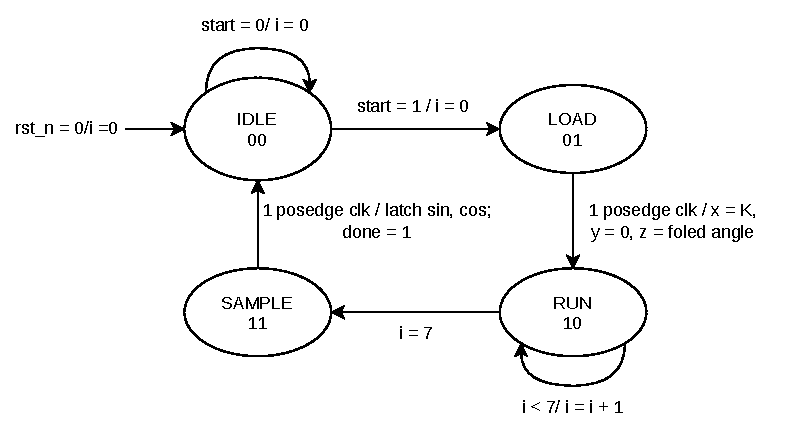
\includegraphics[width=0.92\textwidth]{figures/fsm_diag.pdf}}

\texttt{rst\_n} thấp đưa \texttt{state} về 00, \texttt{i} về 0 và \texttt{done} về 0. Ở \texttt{IDLE}, \texttt{start} bằng 0 thì máy ở lại và \texttt{i} giữ nguyên. \texttt{start} bằng 1 thì nhịp sau là \texttt{LOAD} và \texttt{i} về 0. \texttt{LOAD} kéo dài một \texttt{clk} và luôn sang \texttt{RUN}.

Ở \texttt{RUN}, \texttt{i} nhỏ hơn 7 thì máy ở lại và \texttt{i} tăng 1. \texttt{i} bằng 7 thì nhịp sau là \texttt{SAMPLE} và \texttt{i} giữ nguyên. \texttt{SAMPLE} kéo dài một \texttt{clk} và luôn về \texttt{IDLE}. \texttt{done} bằng 1 ở \texttt{IDLE} ngay sau \texttt{SAMPLE}.

\texttt{RUN} chiếm tám cạnh \texttt{clk}, nên một vòng sau \texttt{start} là một \texttt{LOAD}, tám \texttt{RUN} và một \texttt{SAMPLE}. Cạnh ra khỏi \texttt{LOAD} ghi \texttt{K} vào \texttt{x}, 0 vào \texttt{y}, góc đã gấp vào \texttt{z}, cùng \texttt{sign\_sin} và \texttt{sign\_cos}. Cạnh ra khỏi \texttt{SAMPLE} ghi \texttt{sin} và \texttt{cos}. Bước \texttt{i} bằng 7 không đổi \texttt{z} vì \texttt{alpha} bằng 0.

\section{Thiết kế RTL}

\subsection{Vị trí của mục}

Lõi chia thành khối điều khiển và khối xử lý. Khối điều khiển giữ bốn trạng thái. Khối xử lý giữ đường \texttt{x}, \texttt{y} và \texttt{z}. Số cell và slack bắt đầu từ Mục 4. Mã đầy đủ nằm ở Phụ lục A.

\subsection{Sơ đồ khối}

Ba hình sau được chụp từ schematic editor của thiết kế \texttt{cordic}. Slide \texttt{top} là cả lõi, với khối xử lý cạnh khối điều khiển. Slide \texttt{pu} là đường \texttt{x}, \texttt{y} và \texttt{z}. Slide \texttt{cu} là bốn trạng thái cùng các thanh ghi kết quả.

\figframe{Slide \texttt{top}: lõi \texttt{cordic}, khối xử lý cạnh khối điều khiển.}{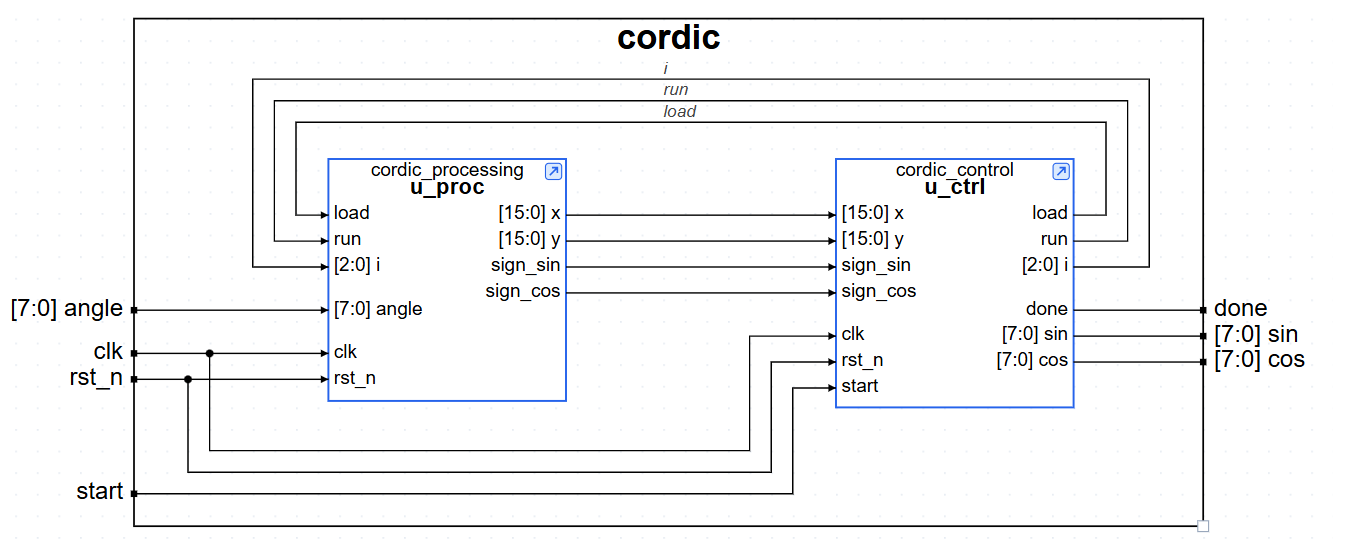
\includegraphics[width=0.92\textwidth]{figures/top.png}}
\figframe{Slide \texttt{pu}: đường \texttt{x}, \texttt{y} và \texttt{z} trong khối xử lý.}{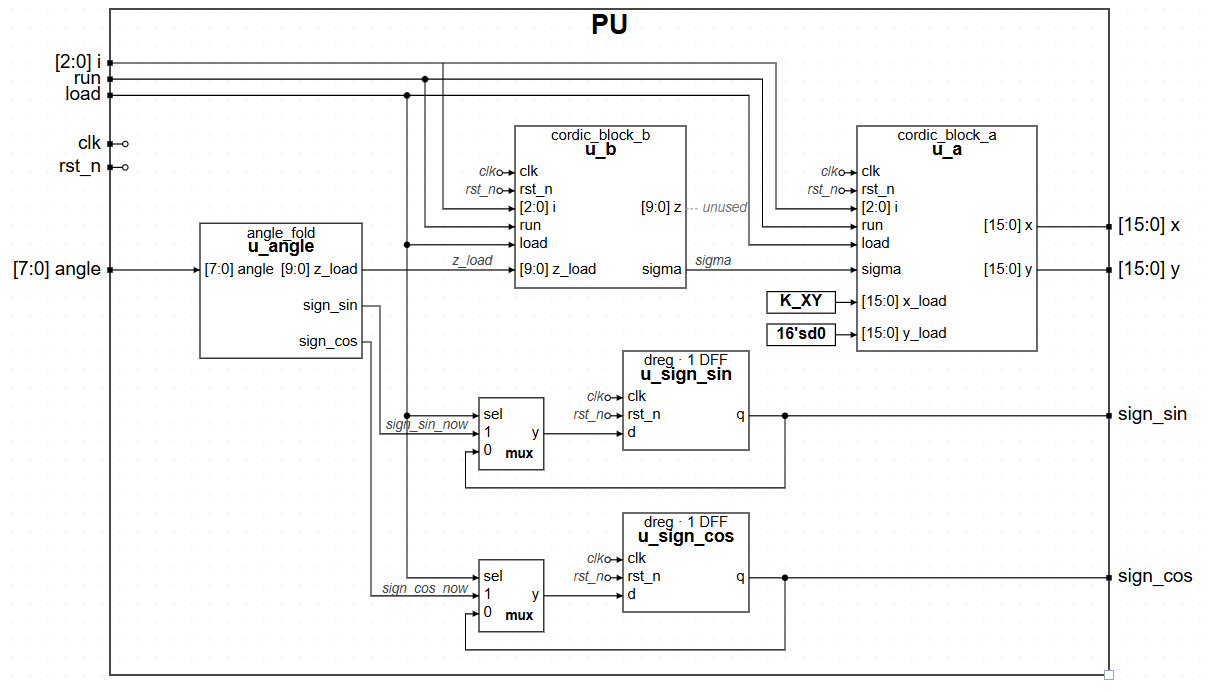
\includegraphics[width=0.92\textwidth]{figures/pu.png}}
\figframe{Slide \texttt{cu}: bốn trạng thái và các thanh ghi kết quả.}{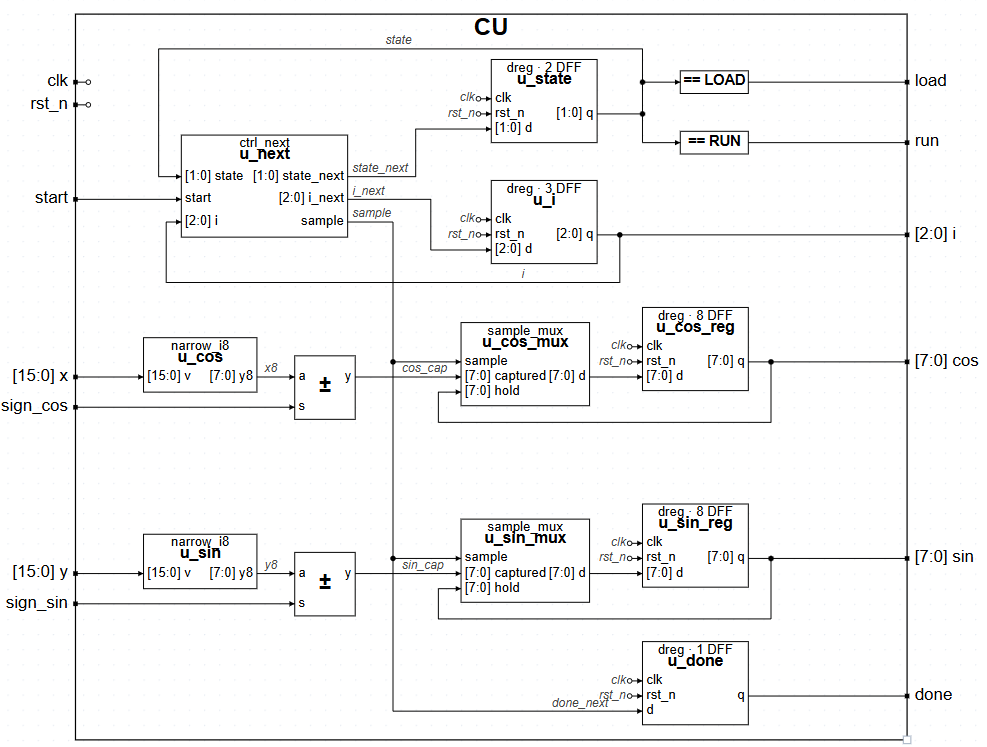
\includegraphics[width=0.92\textwidth]{figures/cu.png}}

\subsection{Quyết định thiết kế}

Bảng 2.1 ghi bốn quyết định của lõi. Phép quay đi bằng tám bước cộng, trừ và dịch trên một bộ cộng. Một phép nhân rộng làm cùng việc trong một nhịp. Phép đó cần cell nhân, nên thiết kế đổi cell nhân lấy thêm nhịp \texttt{clk}. \texttt{x} và \texttt{y} rộng 16 bit. \texttt{K} bằng 9949 không nằm trong 8 bit. Đường 8 bit không chứa được giá trị đầu của phép quay.

Góc vào được gấp về một phần tư trước khi quay. Một đường dữ liệu vì thế phủ cả vòng, và bốn mạch quay song song không có trong sơ đồ. Bốn trạng thái \texttt{IDLE}, \texttt{LOAD}, \texttt{RUN} và \texttt{SAMPLE} dùng lại một bộ cộng trong tám nhịp. Trải tám bước thành mạch tổ hợp sẽ đặt nhiều bộ cộng vào cùng một nhịp.

\noindent\textbf{Bảng 2.1 — Các quyết định thiết kế}

\begin{tabularx}{\textwidth}{|c|Y|Y|Y|}
\hline
\# & Quyết định & Phương án khác đã cân nhắc & Lý do chọn \\ \hline
1 & tám bước cộng, trừ, dịch & một phép nhân rộng & bỏ cell nhân, đổi lấy nhiều nhịp \\ \hline
2 & \texttt{x}, \texttt{y} 16 bit & \texttt{x}, \texttt{y} 8 bit & \texttt{K} \(= 9949\) không nằm trong 8 bit \\ \hline
3 & gấp góc về một phần tư & bốn mạch quay song song & một đường dữ liệu cho cả vòng \\ \hline
4 & bốn trạng thái, dùng lại bộ cộng & trải tám bước thành mạch tổ hợp & một bộ cộng, tám nhịp \\ \hline
\end{tabularx}

\subsection{Đoạn cốt lõi}

Trên slide \texttt{cu}, \texttt{u\_next} là hàm \texttt{ctrl\_next} và \texttt{u\_state} là thanh ghi 2 bit của \texttt{state}. \texttt{u\_i} là thanh ghi 3 bit của \texttt{i}. Hàm này đọc \texttt{state}, \texttt{i} và \texttt{start}, rồi ghi \texttt{state\_next} cùng \texttt{i\_next}. \texttt{eq\_load} kéo \texttt{load} lên 1 khi \texttt{state} là \texttt{LOAD}. \texttt{eq\_run} kéo \texttt{run} lên 1 khi \texttt{state} là \texttt{RUN}.

\texttt{axis\_mux}, \texttt{addsub\_block} và \texttt{axis\_reg} nằm trong \texttt{cordic\_cells.v}. \texttt{sel} của \texttt{axis\_mux} là \{\texttt{load}, \texttt{run}\}. \texttt{load} chọn giá trị nạp. \texttt{run} chọn giá trị vừa quay. Cả hai bằng 0 thì mux giữ thanh ghi. \texttt{addsub\_block} cộng khi \texttt{sigma} khớp \texttt{add\_on\_sigma}, và trừ khi hai tín hiệu đó khác nhau.

Trên slide \texttt{pu}, \texttt{u\_b} cập nhật \texttt{z}. \texttt{u\_angle} gấp \texttt{angle} thành \texttt{z\_load}. Khi \texttt{load} bằng 1, mux của \texttt{u\_b} lấy \texttt{z\_load}. Khi \texttt{run} bằng 1, \texttt{addsub\_block} với \texttt{add\_on\_sigma} bằng 0 trừ \texttt{alpha} khỏi \texttt{z} nếu \texttt{sigma} bằng 1, và cộng \texttt{alpha} nếu \texttt{sigma} bằng 0. \texttt{atan\_lut} chọn \texttt{alpha} theo \texttt{i}. \texttt{axis\_reg} ghi kết quả vào \texttt{z} ở cạnh \texttt{clk}.

\texttt{u\_a} cập nhật \texttt{x} và \texttt{y} bằng \texttt{shift\_block}. \texttt{sigma} bằng 1 thì \texttt{x} trừ \(\texttt{y} \gg \texttt{i}\) và \texttt{y} cộng \(\texttt{x} \gg \texttt{i}\). \texttt{add\_on\_sigma} của đường \texttt{x} là 0, và của đường \texttt{y} là 1. Khi \texttt{load} bằng 1, \texttt{x} nhận 9949 từ \texttt{const\_K\_XY} và \texttt{y} nhận 0 từ \texttt{const\_16\_sd0}.

Phụ lục A chép nguyên văn các file của lõi, của vỏ chân và của testbench.

\section{Kiểm chứng chức năng}

\subsection{Vì sao chọn từng ca}

Bảng 3.1 có mười mã, chia bốn nhóm. Năm mã đầu phủ \(0^\circ\), \(30^\circ\), \(45^\circ\), \(60^\circ\) và \(90^\circ\). Hai mã tự chọn là 96 và 255. Mã 96 là \(135^\circ\). Sau khi gấp, \texttt{z\_load} bằng 32, cùng giá trị của mã 32, và chỉ \texttt{sign\_cos} bằng 1, nên ca này kiểm tra dấu cosine trên đúng phép quay của \(45^\circ\). Mã 255 là biên, vì nó đứng một bước trước đủ một vòng. Ba mã 128, 192 và 224 thêm một mã cho mỗi phần tư còn lại.

\subsection{Giá trị mong đợi}

Kỳ vọng được tính trong \texttt{error\_table.py} trước khi trừ số của mạch. Với mã \(n\),

\[
\theta = 2\pi n / 256, \qquad \mathrm{ideal} = \mathrm{round}(128\sin\theta).
\]

Cosine dùng cùng công thức với \(\cos\theta\). Mỗi kết quả bị kẹp vào \(-128\) đến \(127\).

\subsection{Hai ca tự chọn}

Mã 96 là \(135^\circ\) đúng. \texttt{z\_load} sau gấp bằng 32, như mã 32. \texttt{sign\_sin} giữ 0 và \texttt{sign\_cos} bằng 1. Phép quay trong \texttt{u\_b} vì thế đi lại đường của \(45^\circ\), và \texttt{SAMPLE} chỉ đổi dấu \texttt{cos}. Mã 255 là \(358{,}59^\circ\), một bước trước đủ một vòng.

\subsection{Dạng sóng}

\texttt{tb\_gtkwave.v} chạy một lần tính với mã góc vào 32. Mã này không phải \(32^\circ\). Góc lấy mẫu ban đầu là \(32 \times 360^\circ/256 = 45^\circ\).

Hình~\ref{fig:gtk} là sóng của lần tính đó. Ảnh gồm \texttt{state}, \texttt{i}, \texttt{x}, \texttt{y}, \texttt{z}, \texttt{sigma}, \texttt{sin}, \texttt{cos} và \texttt{done}. Bảng dưới là phép tính tay của tám bước \texttt{RUN}. Mỗi hàng \texttt{RUN} ghi giá trị ở đầu bước, và hàng kế là kết quả của bước đó. Khi \texttt{sigma} \(= 1\), tức \texttt{z} \(\ge 0\), một bước là

\[
\texttt{x} \leftarrow \texttt{x} - (\texttt{y} \gg \texttt{i}),\quad
\texttt{y} \leftarrow \texttt{y} + (\texttt{x} \gg \texttt{i}),\quad
\texttt{z} \leftarrow \texttt{z} - \texttt{alpha}.
\]

Khi \texttt{sigma} \(= 0\), cả ba phép đổi chiều. Tám giá trị \texttt{alpha} là 32, 19, 10, 5, 3, 1, 1 và 0.

\begin{center}
\scriptsize
\begin{tabular}{|l|c|c|r|r|r|l|}
\hline
Trạng thái & \texttt{i} & \texttt{sigma} & \texttt{x} & \texttt{y} & \texttt{z} & Việc của bước \\ \hline
\texttt{IDLE}, sau \texttt{rst\_n} & 0 & 1 & 0 & 0 & 0 & \texttt{sin} và \texttt{cos} bằng 0 \\ \hline
\texttt{LOAD} & 0 & 1 & 0 & 0 & 0 & \texttt{start} còn cao \\ \hline
\texttt{RUN} & 0 & 1 & 9949 & 0 & 32 & vừa ghi \texttt{K} và \texttt{z} từ mã góc vào \\ \hline
\texttt{RUN} & 1 & 1 & 9949 & 9949 & 0 & xong bước 0 \\ \hline
\texttt{RUN} & 2 & 0 & 4975 & 14923 & $-19$ & xong bước 1 \\ \hline
\texttt{RUN} & 3 & 0 & 8705 & 13680 & $-9$ & xong bước 2 \\ \hline
\texttt{RUN} & 4 & 0 & 10415 & 12592 & $-4$ & xong bước 3 \\ \hline
\texttt{RUN} & 5 & 0 & 11202 & 11942 & $-1$ & xong bước 4 \\ \hline
\texttt{RUN} & 6 & 1 & 11575 & 11592 & 0 & xong bước 5 \\ \hline
\texttt{RUN} & 7 & 0 & 11394 & 11772 & $-1$ & xong bước 6 \\ \hline
\texttt{SAMPLE} & 7 & 0 & 11485 & 11683 & $-1$ & xong bước 7 \\ \hline
\texttt{IDLE} & 7 & 0 & 11485 & 11683 & $-1$ & \texttt{done}=1, \texttt{sin} 91, \texttt{cos} 89 \\ \hline
\end{tabular}
\end{center}

Ở nhịp \texttt{done}, sau trạng thái \texttt{SAMPLE}, \texttt{sin} và \texttt{cos} là \texttt{x} và \texttt{y} dịch phải 7 bit. \(11683 / 128 = 91{,}27\) và \texttt{sin} làm tròn thành 91. \(11485 / 128 = 89{,}73\) và \texttt{cos} làm tròn thành 89.

Giá trị thật của \(45^\circ\) là \(\sin = \cos = 0{,}70710678\). Cùng thang 128 thì

\[
128 \times 0{,}70710678 = 90{,}51,
\]

và 90{,}51 làm tròn thành mã 91. \texttt{sin} trên ảnh khớp mã này. \texttt{cos} lệch 2 mã, và lệch đó là sai số của tám bước.

Trên ảnh, con trỏ đứng ở nhịp \texttt{done}. \texttt{state} là 00, \texttt{i} là 7, \texttt{x} là 11485 và \texttt{y} là 11683. \texttt{sin} là 91 và \texttt{cos} là 89. \texttt{z} hiện 1023 vì cửa sổ vẽ số không dấu. Cùng 10 bit đó, đọc có dấu, là \(-1\), đúng \texttt{z} ở hàng trạng thái \texttt{SAMPLE}.

\figframe{GTKWave của mã 32, tại nhịp \texttt{done}.\label{fig:gtk}}{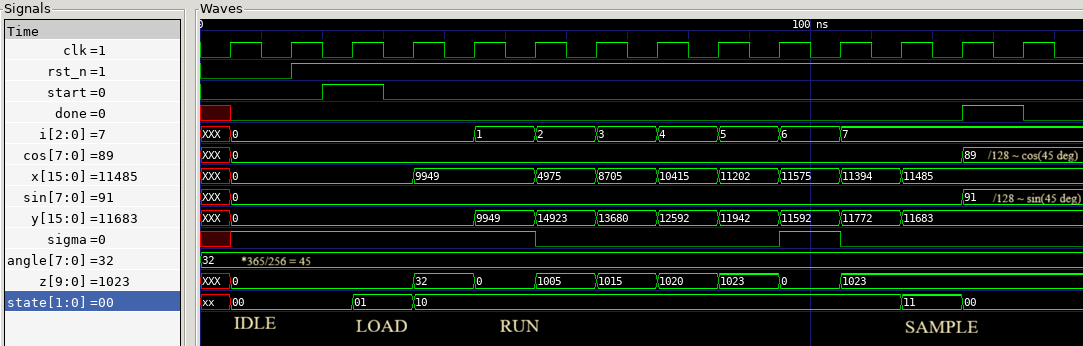
\includegraphics[width=0.96\textwidth]{figures/gtk_wave.png}}

\subsection{Ca từng đỏ}

Hai testbench (TB) đã lưu đều in dòng đạt (PASS) trên RTL gốc. Dòng của lõi là \texttt{I05 RTL TB PASS}. Dòng của vỏ chân (PIN SHELL) là \texttt{I05 PIN SHELL PASS}. Phép phá mạch dùng bản sao của \texttt{cordic\_control.v} và bỏ dấu cosine: \texttt{cos\_cap} bằng \texttt{x8}, không còn \texttt{sign\_cos ? -x8 : x8}. Sáu cặp và dải \(\pm 4\) của \texttt{tb\_cordic.v} giữ nguyên. Mã 0 và mã 64 còn trong dải. Mã 128 làm cosine thành 127, trong khi mong đợi là \(-128\), và bench dừng bằng \texttt{\$fatal}. Ba mã sau, 192, 32 và 224, vẫn trong dải khi chạy tiếp cùng luật. File gốc không đổi.

\noindent\textbf{Bảng 3.1 — Ca kiểm thử và kết quả}

{\small
\begin{tabularx}{\textwidth}{|c|Y|Y|Y|Y|Y|Y|}
\hline
\# & Ca kiểm thử & Đầu vào & Mong đợi & Thu được & Đạt & Vì sao chọn ca này \\ \hline
1 & \(0^\circ\) & 0 & 0, 127 & $-2$, 127 & có & đầu dải \\ \hline
2 & gần \(30^\circ\) & 21 & 63, 111 & 64, 110 & có & mã gần \(30^\circ\) \\ \hline
3 & \(45^\circ\) & 32 & 91, 91 & 91, 89 & có & đúng mã \\ \hline
4 & gần \(60^\circ\) & 43 & 111, 63 & 113, 59 & có & mã gần \(60^\circ\) \\ \hline
5 & \(90^\circ\) & 64 & 127, 0 & 127, 4 & có & biên sai số cosine bằng 4 \\ \hline
6 & \(135^\circ\), tự chọn & 96 & 91, $-91$ & 91, $-89$ & có & cùng \texttt{z\_load} với \(45^\circ\), đảo \texttt{sign\_cos} \\ \hline
7 & \(180^\circ\) & 128 & 0, $-128$ & 2, $-127$ & có & phần tư thứ ba \\ \hline
8 & \(270^\circ\) & 192 & $-128$, 0 & $-127$, $-4$ & có & phần tư thứ tư \\ \hline
9 & \(315^\circ\) & 224 & $-91$, 91 & $-91$, 89 & có & đối của \(45^\circ\) \\ \hline
10 & biên, tự chọn & 255 & $-3$, 127 & $-4$, 127 & có & một bước trước đủ vòng \\ \hline
\end{tabularx}
}

Trong Bảng 3.1, mỗi ô ghi sine trước rồi cosine sau. Bench sáu cặp chấp nhận lệch trong \(\pm 4\). Trên mười mã này, lệch sine lớn nhất là 2 và lệch cosine lớn nhất là 4.

\noindent\textbf{Bảng 3.2 — Phép thử phá mạch (bắt buộc)}

\begin{tabularx}{\textwidth}{|Y|Y|Y|Y|}
\hline
Lỗi cố tình tạo ra & Số ca chuyển sang đỏ & Ca nào đỏ & Kết luận về chất lượng testbench \\ \hline
bỏ \texttt{sign\_cos} ở \texttt{cos\_cap} & 1 / 6 & mã 128 & bench dừng khi cosine thành 127 thay vì \(-128\) \\ \hline
\end{tabularx}

\section{Kết quả tổng hợp}

\subsection{Ước lượng trước khi đối chiếu}

Số flip-flop được đếm từ RTL trước khi map, và tổng là 66 bit. Map sky130 của lần chạy \texttt{RUN\_2026.\allowbreak 10.03\_\allowbreak 09.21.28} có 66 cell \texttt{dfrtp\_1}. Bảng 4.1 đặt ước lượng cạnh số thật.

\subsection{Đối chiếu flip-flop}

66 bit khai báo gồm \texttt{x} và \texttt{y} 16 bit mỗi thanh ghi, cùng \texttt{z} 10 bit. \texttt{sin} và \texttt{cos} chiếm 8 bit mỗi thanh ghi. \texttt{i} chiếm 3 bit, \texttt{state} chiếm 2 bit, \texttt{done} chiếm 1 bit, và \texttt{sign\_sin} với \texttt{sign\_cos} chiếm phần còn lại. Mỗi bit thành một cell \texttt{dfrtp}: một flip-flop lấy dữ liệu ở cạnh lên của \texttt{clk} và xóa về 0 khi \texttt{rst\_n} thấp. Hậu tố \texttt{\_1} hay \texttt{\_2} là sức kéo của cổng ra, không phải số bit. Map ra đúng 66 flip-flop. Lệch bằng 0, nên không có thanh ghi thừa và cũng không mất thanh ghi.

\subsection{Loại cell}

File \texttt{1-synthesis.AREA\_0.stat.rpt} ghi diện tích lõi lúc map là \(7553{,}49\,\mu\mathrm{m}^{2}\) và 672 cell. File đó đếm từng tên cell, không nhân số cell với diện tích một cell, nên chưa chỉ được loại nào chiếm nhiều \(\mu\mathrm{m}^{2}\) nhất. Tên lặp nhiều nhất trong file này là flip-flop, 66 lần. Bản đếm 734 cell ở bước Yosys trước flow có 22 cell \texttt{maj3\_1}. Cổng \texttt{maj3} ra mức 1 khi ít nhất hai trong ba đầu vào bằng 1. Yosys chọn cổng này lúc map phép cộng và phần logic còn lại. Không có cell nhân và không có bộ nhớ. Bảng 4.2 tách bốn loại cell đếm được.

\noindent\textbf{Bảng 4.1 — Số liệu tổng hợp}

\begin{tabularx}{\textwidth}{|Y|Y|Y|Y|}
\hline
Chỉ số & Ước lượng trước khi chạy & Kết quả thật & Chênh lệch và giải thích \\ \hline
Tổng số standard cell & không ước lượng trước & 734 & số sau map sky130 \\ \hline
Số flip-flop & 66 bit từ RTL & 66 \texttt{dfrtp\_1} & lệch 0 \\ \hline
Diện tích cell ($\mu$m$^{2}$) & — & 7553{,}49 & tổng lúc map, chưa tách theo loại \\ \hline
Hệ số sử dụng (\%) & 45, mục tiêu đặt & 23{,}41 lúc đặt & \texttt{Final\_Util} \(= -1\), chưa có số sau đi dây \\ \hline
\end{tabularx}

Bốn số cell là bốn bước khác nhau, không phải bốn lần đếm cùng một tập. 734 là số cell sau map sky130 ở bước Yosys trước flow. 672 là số cell trong \texttt{1-synthesis.AREA\_0.stat.rpt} của chính lần chạy, và ở file đó flip-flop mang tên \texttt{dfrtp\_2}, vẫn 66 lần. 755 là số cell đã đặt lên đế, không kể filler. 3901 là 755 cộng 3146 cell không tính toán.

Một hàng standard cell có hai ray. \texttt{VPWR} là ray nguồn. \texttt{VGND} là ray đất. Cell logic, gồm \texttt{dfrtp} và \texttt{maj3}, nằm giữa hai ray và làm tính toán. Ba cell còn lại không tính \texttt{sin} hay \texttt{cos}. \texttt{config.tcl} của thiết kế không bật hai công tắc này. OpenLane ghi mặc định \texttt{RUN\_TAP\_DECAP\_INSERTION} và \texttt{RUN\_FILL\_INSERTION} bằng 1 vào \texttt{config.tcl} của lần chạy, nên công cụ tự chèn chúng sau khi đặt cell logic. Hình~\ref{fig:row} đối chiếu một hàng còn lỗ với hàng đã chèn. Đó là sơ đồ, không phải ảnh cắt từ file GDSII.

Tap, tên \texttt{tapvpwrvgnd\_1}, nối giếng n với \texttt{VPWR} và đế p với \texttt{VGND}. Thiếu tap thì giếng nổi, transistor dễ latch-up, và luật khoảng cách giếng của sky130 bị phạm. Cách đặt thông thường là một lưới, không phải một tap cho mỗi cổng. File \texttt{config.tcl} của thiết kế không ghi khoảng này. OpenLane lấy mặc định của sky130 và chép vào \texttt{config.tcl} của lần chạy: \texttt{FP\_TAPCELL\_DIST} bằng 13, tức một tap cách tap kế khoảng \(13\,\mu\mathrm{m}\). Netlist cuối có 469 tap.

Decap là tụ giữa hai ray. Khi nhiều cổng đổi mức cùng lúc, tụ này cấp điện tích tại chỗ, nên điện áp trên ray sụt ít hơn. Thiếu decap thì sụt áp trên ray tăng. Công cụ không vẽ tay từng tụ. Biến \texttt{DECAP\_CELL} liệt kê từ rộng đến hẹp: \texttt{decap\_12}, \texttt{decap\_8}, \texttt{decap\_6}, \texttt{decap\_4}, rồi \texttt{decap\_3}. Chỗ trống nhận bản rộng nhất còn vừa. Vì vậy \texttt{decap\_12} chiếm 1239 trong 2103 decap.

Filler, tên \texttt{fill\_1} và \texttt{fill\_2}, không có chân logic và gần như không có điện dung. Nó chỉ bịt ô rộng 1 hoặc 2 mà decap không vừa, để ray và giếng không đứt đoạn. Bỏ filler thì DRC mật độ và tính liên tục của ray hỏng, dù chức năng RTL không đổi. Netlist cuối có 574 filler, gồm \texttt{fill\_1} 432 và \texttt{fill\_2} 142. Không cell nào trong ba nhóm này giữ \texttt{x}, \texttt{y} hay \texttt{z}.

\figframe{Cách chèn trên một hàng. Hàng trên còn lỗ: giếng chưa được tap buộc, chỗ trống làm ray đứt. Hàng dưới là thứ tự của lần chạy: tap theo lưới \(13\,\mu\mathrm{m}\), decap rộng nhất còn vừa, filler bịt ô còn lại. Đây không phải ảnh của đế \texttt{cordic}.\label{fig:row}}{%
\begin{tikzpicture}[x=1.05cm,y=0.72cm,font=\scriptsize]
  \node[anchor=west] at (0,3.55) {chưa chèn};
  \draw[thick] (0,2.55) -- (1.7,2.55);
  \draw[thick,dashed] (1.7,2.55) -- (4.5,2.55);
  \draw[thick] (4.5,2.55) -- (7.6,2.55);
  \node[above] at (3.8,2.55) {\texttt{VPWR} đứt};
  \draw[fill=blue!8] (0.15,0.85) rectangle (1.7,2.2);
  \node at (0.92,1.52) {logic};
  \draw[dashed] (1.85,0.85) rectangle (4.35,2.2);
  \node[align=center] at (3.1,1.52) {lỗ\\giếng nổi};
  \draw[fill=blue!8] (4.5,0.85) rectangle (6.05,2.2);
  \node at (5.27,1.52) {logic};
  \draw[dashed] (6.2,0.85) rectangle (7.45,2.2);
  \draw[thick] (0,0.45) -- (7.6,0.45);
  \node[below] at (3.8,0.45) {\texttt{VGND}};
  \node[anchor=west] at (0,-0.55) {đã chèn};
  \draw[thick] (0,-1.35) -- (7.6,-1.35);
  \node[above] at (3.8,-1.35) {\texttt{VPWR} liên tục};
  \draw[fill=blue!8] (0.15,-3.05) rectangle (1.55,-1.7);
  \node at (0.85,-2.37) {logic};
  \draw[fill=orange!25] (1.7,-3.05) rectangle (2.7,-1.7);
  \node[align=center] at (2.2,-2.37) {tap\\13};
  \draw[fill=green!16] (2.85,-3.05) rectangle (5.15,-1.7);
  \node at (4.0,-2.37) {\texttt{decap\_12}};
  \draw[fill=gray!22] (5.3,-3.05) rectangle (6.05,-1.7);
  \node at (5.67,-2.37) {\texttt{fill}};
  \draw[fill=blue!8] (6.2,-3.05) rectangle (7.45,-1.7);
  \node at (6.82,-2.37) {logic};
  \draw[thick] (0,-3.45) -- (7.6,-3.45);
  \node[below] at (3.8,-3.45) {\texttt{VGND}};
\end{tikzpicture}}
% Optional photo of a cell row: save as report/figures/cell_row.png
\optfig{figures/cell_row.png}{Ảnh một hàng standard cell: logic, filler, tap và decap giữa hai ray. Ảnh của người viết, không phải slide của khóa học.}

\subsection{Những gì thiết kế đặt vào chuỗi nhịp}

Chuỗi một lần tính do RTL đặt: một nhịp \texttt{LOAD}, tám nhịp \texttt{RUN} và một nhịp \texttt{SAMPLE}. Đó là mười cạnh \texttt{clk}. Hình~\ref{fig:seq} gắn mỗi cạnh với dòng đã ghi trong file thiết kế. Tap, decap và filler không nằm trên chuỗi này.

\texttt{CLOCK\_PERIOD} bằng 10 ns là thời gian cho phép của từng cạnh, không phải của cả mười cạnh. Đường từ một thanh ghi tới thanh ghi kế phải xong trong 10 ns đó. Slack setup \(4{,}73\,\mathrm{ns}\) là phần còn dư bên trong một cạnh, không phải dư của tám bước \texttt{RUN}. Mười cạnh đặt cạnh nhau là \(10 \times 10\,\mathrm{ns} = 100\,\mathrm{ns}\) theo ràng buộc. Đó không phải thời gian đo trên chip.

\texttt{IO\_PCT} bằng 0{,}2 dành 2 ns ở biên của cùng cạnh đó. Ở cạnh vào \texttt{LOAD}, mã góc và \texttt{start} được coi là đã tới chân sau 2 ns, nên phần trong lõi còn 8 ns. Ở cạnh ra khỏi \texttt{SAMPLE}, \texttt{sin} và \texttt{cos} phải sẵn sàng trước 2 ns cho mạch ngoài. \texttt{SYNTH\_ADDER\_TYPE} bằng \texttt{YOSYS} giữ tám nhịp \texttt{RUN} là cộng, trừ và dịch. Vì vậy bảng cell không có bộ nhân. \texttt{SYNTH\_STRATEGY} bằng \texttt{AREA 0} chỉ bảo Yosys map ít cell hơn. Nó không đổi số nhịp.

Đế \(200\,\mu\mathrm{m}\) và mật độ 0{,}45 không đổi chuỗi. Hai dòng đó chỉ chừa chỗ cho cùng 66 thanh ghi. Khoảng tap, danh sách decap và hai công tắc filler không có trong \texttt{config.tcl} của thiết kế. Flow không dừng giữa chừng để sửa một filler hay một slack. Muốn chuỗi ngắn hơn thì sửa RTL. Muốn mỗi cạnh ngắn hơn thì sửa \texttt{CLOCK\_PERIOD} rồi chạy lại. Lần chạy đã nộp không làm cả hai.

\figframe{Mười cạnh của một lần tính. Mỗi cạnh là một \texttt{CLOCK\_PERIOD} bằng 10 ns do \texttt{config.tcl} đặt. Trễ chân 2 ns nằm ở cạnh \texttt{LOAD} và ở cạnh ra khỏi \texttt{SAMPLE}.\label{fig:seq}}{%
\begin{tikzpicture}[x=0.95cm,y=0.7cm,font=\scriptsize]
  \draw[thick,->] (0,0) -- (10.6,0);
  \foreach \x/\name in {0.4/LOAD,1.4/0,2.4/1,3.4/2,4.4/3,5.4/4,6.4/5,7.4/6,8.4/7,9.4/SAMPLE} {
    \draw (\x,0.08) -- (\x,-0.08);
  }
  \node[above] at (0.4,0.1) {\texttt{LOAD}};
  \node[above] at (4.9,0.1) {tám \texttt{RUN}, \texttt{i} = 0\ldots7};
  \node[above] at (9.4,0.1) {\texttt{SAMPLE}};
  \node[below,align=center] at (0.4,-0.15) {góc, \texttt{start}\\trễ chân 2 ns};
  \node[below] at (4.9,-0.15) {mỗi cạnh 10 ns};
  \node[below,align=center] at (9.4,-0.15) {\texttt{sin}, \texttt{cos}\\sẵn trước 2 ns};
\end{tikzpicture}}

\noindent\textbf{Bảng 4.2 — Phân loại cell}

\begin{tabularx}{\textwidth}{|Y|Y|Y|}
\hline
Loại cell & Số lượng & Vai trò trong mạch \\ \hline
\texttt{dfrtp\_1} & 66 & thanh ghi của \texttt{x}, \texttt{y}, \texttt{z}, trạng thái và kết quả \\ \hline
\texttt{maj3\_1} & 22 & cổng majority sau map, không phải bộ nhân \\ \hline
bộ nhân & 0 & tám bước không nhân \\ \hline
bộ nhớ & 0 & không có bảng sine \\ \hline
\end{tabularx}

\section{Kết quả phân tích thời gian}

\subsection{Setup và hold}

Ràng buộc chu kỳ là 10 ns và trễ chân là 2 ns. Số thời gian dưới đây lấy từ bước signoff, tức bước kiểm sau khi dây đã đi. File là \texttt{31-rcx\_sta}. Chữ rcx là phép rút điện trở và tụ của chính những dây đó. Static timing analysis (STA) trên file này dùng điện trở và tụ đã rút, không dùng độ trễ ước lượng trước khi đi dây.

Worst negative slack (WNS) và total negative slack (TNS) trong \texttt{metrics.csv} đều bằng 0. WNS bằng 0 chỉ có nghĩa không có đường nào trễ quá chu kỳ. Nó không phải độ dư của đường chậm nhất. Trong \texttt{31-rcx\_sta.summary.rpt}, slack setup lớn nhất là \(4{,}73\,\mathrm{ns}\) và được ghi MET, tức còn trong hạn. Slack hold nhỏ nhất là \(0{,}29\,\mathrm{ns}\), cũng MET. Hold là đường ngắn nhất: dữ liệu không được tới chân D quá sớm so với cùng cạnh \texttt{clk}.

Slack của một đường là hạn cho phép trừ thời điểm dữ liệu tới. Trên đường setup chậm nhất, hạn là \(10{,}08\,\mathrm{ns}\) và dữ liệu tới lúc \(5{,}35\,\mathrm{ns}\), nên slack bằng \(4{,}73\,\mathrm{ns}\). Trên đường hold ngắn nhất, dữ liệu tới lúc \(0{,}92\,\mathrm{ns}\) và hạn là \(0{,}63\,\mathrm{ns}\), nên slack bằng \(0{,}29\,\mathrm{ns}\). Số dương nghĩa là đường còn trong hạn. WNS bằng 0 vì công cụ chỉ ghi phần âm, và ở đây không có phần âm.

% Optional slack diagram: save as report/figures/slack.png
\optfig{figures/slack.png}{Slack là hạn cho phép trừ thời điểm dữ liệu tới. Ảnh minh họa của người viết cho đường setup và đường hold của lần chạy này.}

\subsection{Đường tới hạn}

Đường setup chậm nhất trong \texttt{31-rcx\_sta.max.rpt} đi từ flip-flop \texttt{\_1240\_} đến flip-flop \texttt{\_1226\_}. Cổng Q của \texttt{\_1240\_} là bit \texttt{u\_ctrl.i[0]}, tức bit 0 của bộ đếm vòng trong khối điều khiển. Cổng Q của \texttt{\_1226\_} mang tên net \texttt{u\_ctrl.u\_sin.t[10]}, một dây bên trong khối thu hẹp \texttt{y} thành \texttt{sin}. Dữ liệu tới chân D lúc \(5{,}35\,\mathrm{ns}\). Hạn cho phép là \(10{,}08\,\mathrm{ns}\). Hiệu hai số là slack \(4{,}73\,\mathrm{ns}\).

Từ Q đến D có 15 cell tổ hợp: một đệm, \texttt{mux4}, \texttt{mux2}, \texttt{or4}, một đệm nữa, \texttt{o31a}, hai \texttt{xor2}, \texttt{and2b}, \texttt{a311o}, \texttt{a211oi}, \texttt{nor2}, \texttt{o211a}, \texttt{or3} và \texttt{a32o}. Đường này nằm trong khối điều khiển, không phải bộ cộng 16 bit của \texttt{x} và \texttt{y}.

Đường hold ngắn nhất trong \texttt{31-rcx\_sta.min.rpt} xuất phát và kết thúc cùng flip-flop \texttt{\_1213\_}. Dây ra là \texttt{u\_ctrl.u\_sin.v[2]}. Dữ liệu tới sau \(0{,}92\,\mathrm{ns}\), hạn hold là \(0{,}63\,\mathrm{ns}\), slack \(0{,}29\,\mathrm{ns}\).

% Optional path drawing: save as report/figures/setup_path.png
\optfig{figures/setup_path.png}{Đường setup từ \texttt{\_1240\_} (\texttt{u\_ctrl.i[0]}) tới \texttt{\_1226\_}. Ảnh của người viết cho lần chạy này.}

\subsection{Tần số ước tính}

\(100\,\mathrm{MHz}\) là \(1/10\,\mathrm{ns}\), tức tần số của ràng buộc. Vì slack setup còn \(4{,}73\,\mathrm{ns}\), một ước lượng chu kỳ ngắn hơn là \(10 - 4{,}73 = 5{,}27\,\mathrm{ns}\), khoảng \(190\,\mathrm{MHz}\). Công cụ vẫn ghi tần số gợi ý \(100\,\mathrm{MHz}\), vì nó chỉ hạ gợi ý khi WNS âm. Cả hai số đều là mô hình STA, không phải tần số đo trên chip. Bảng 5.1 chép chu kỳ, slack setup, slack hold và tần số của ràng buộc.

\subsection{Mạch có thanh ghi}

Mạch có thanh ghi, nên STA có đường từ thanh ghi này đến thanh ghi kia. Slack setup \(4{,}73\,\mathrm{ns}\) và slack hold \(0{,}29\,\mathrm{ns}\) đều thuộc các đường đó, dưới chu kỳ 10 ns. Mạch này không phải mạch tổ hợp thuần.

\subsection{Không hạ chu kỳ}

WNS không âm dưới chu kỳ 10 ns. Lần chạy đã giữ vẫn là layout duy nhất được trích. Không có lần chạy thứ hai với chu kỳ dài hơn.

\noindent\textbf{Bảng 5.1 — Số liệu thời gian}

\begin{tabularx}{\textwidth}{|Y|Y|Y|Y|}
\hline
Chỉ số & Giá trị & Đạt / Vi phạm & Nhận xét \\ \hline
Chu kỳ ràng buộc (ns) & 10 & — & trễ chân 2 ns \\ \hline
Worst setup slack (ns) & 4{,}73 & đạt, MET & WNS ghi 0 vì không có slack âm \\ \hline
Worst hold slack (ns) & 0{,}29 & đạt, MET & \texttt{31-rcx\_sta.min.rpt} \\ \hline
Tần số của ràng buộc (MHz) & 100 & — & \(f = 1/10\,\mathrm{ns}\), không phải tần số đo \\ \hline
\end{tabularx}

Đệm nhịp \texttt{clkbuf\_\allowbreak 3\_2\_\_f\_clk} kéo 11 tải, trong khi giới hạn của lần chạy là 10. Cảnh báo này không làm WNS thành âm.

\noindent\textbf{Bảng 5.2 — Đường tới hạn}

\begin{tabularx}{\textwidth}{|l|Y|}
\hline
Hạng mục & Nội dung \\ \hline
Điểm xuất phát & \texttt{\_1240\_}, Q là \texttt{u\_ctrl.i[0]} \\ \hline
Điểm kết thúc & \texttt{\_1226\_}, Q là \texttt{u\_ctrl.u\_sin.t[10]} \\ \hline
Đi qua các khối & 15 cell tổ hợp trong khối điều khiển, từ bit \texttt{i} tới đường thu \texttt{sin} \\ \hline
Số tầng logic & 15 cell từ Q đến D \\ \hline
Vì sao chính đường này chậm nhất & dữ liệu tới lúc \(5{,}35\,\mathrm{ns}\), trễ hơn mọi đường setup khác trong file \\ \hline
Một cách cụ thể để rút ngắn nó & cắt bớt tầng mux và xor trên đường từ \texttt{i[0]} tới thanh ghi \texttt{sin} \\ \hline
\end{tabularx}

\section{Công suất và kiểm tra vật lý}

\subsection{Công suất}

\texttt{31-rcx\_sta.power.rpt} ước lượng công suất ở góc điển hình, sau khi đã rút điện trở và tụ của dây. Công suất động gồm hai phần: internal \(2{,}37\times 10^{-3}\,\mathrm{W}\), tức hao bên trong cell khi đổi mức, và switching \(2{,}23\times 10^{-3}\,\mathrm{W}\), tức hao để nạp tụ dây. Công suất tĩnh, tức dòng rò, là \(6{,}07\times 10^{-9}\,\mathrm{W}\). Tổng là \(4{,}59\times 10^{-3}\,\mathrm{W}\). Internal chiếm 51{,}5\% và switching chiếm 48{,}5\%. Rò gần như bằng 0 trong bảng này. Nhóm tổ hợp chiếm 85{,}8\% tổng công suất, nhóm thanh ghi chiếm 14{,}2\%. Đây là ước lượng của mô hình, không phải số đo trên chip.

% Optional power split: save as report/figures/power.png
\optfig{figures/power.png}{Ba phần công suất của lần chạy: internal, switching và dòng rò. Ảnh của người viết.}

\subsection{Luật vẽ và đối chiếu sơ đồ}

Ba phép kiểm hình học của cùng lần chạy đều có số. Magic báo design rule check (DRC) bằng 0, layout versus schematic (LVS) sạch, và kiểm ăng-ten bằng 0. DRC chỉ hỏi hình vẽ có phạm luật vẽ hay không. LVS chỉ hỏi layout có khớp sơ đồ nối hay không. Cả hai phép không đọc sine và cosine.

\subsection{Luật vẽ không chứng minh chức năng}

DRC bằng 0 không có nghĩa mạch tính đúng sine và cosine. Phép này chỉ đếm vi phạm hình học. Chức năng nằm ở Bảng 3.1. Trên mười mã của bảng đó, lệch cosine lớn nhất là 4 mã. Ảnh đế của cùng lần chạy nằm ở mục sau.

\noindent\textbf{Bảng 6.1 — Công suất và kiểm tra vật lý}

\begin{tabularx}{\textwidth}{|Y|Y|Y|}
\hline
Hạng mục & Giá trị / Kết quả & Nhận xét và giới hạn \\ \hline
Công suất động & \(4{,}60\times 10^{-3}\,\mathrm{W}\) & internal \(2{,}37\times 10^{-3}\) cộng switching \(2{,}23\times 10^{-3}\) \\ \hline
Công suất tĩnh (rò) & \(6{,}07\times 10^{-9}\,\mathrm{W}\) & rất nhỏ so với phần động \\ \hline
Tổng công suất & \(4{,}59\times 10^{-3}\,\mathrm{W}\) & góc điển hình, file \texttt{31-rcx\_sta.power.rpt} \\ \hline
DRC & 0 vi phạm & luật hình học, không phải chức năng \\ \hline
LVS & sạch & layout khớp sơ đồ, không phải bảng sai số \\ \hline
ăng-ten & 0 vi phạm & luật ăng-ten của dây, không phải chức năng \\ \hline
\end{tabularx}

\section{Quan sát layout}

\subsection{Ảnh layout}

Hình~\ref{fig:gds} là ảnh hai chiều của file GDSII, lõi \texttt{cordic}, lần chạy đã giữ. Đỉnh của file là \texttt{cordic}. Vỏ \texttt{tt\_um\_cordic} chỉ được mô phỏng và không có trong file này.

\figframe{Ảnh hai chiều của file GDSII, lõi \texttt{cordic}: hàng cell và dây trên đế \(200\,\mu\mathrm{m}\), lần chạy \texttt{RUN\_2026.\allowbreak 10.03\_\allowbreak 09.21.28}.\label{fig:gds}}{\includegraphics[width=0.72\textwidth]{cordic_gds.png}}

Hình~\ref{fig:gdsrows} là cùng đế khi chỉ còn các hàng. Vệt ngang đều nhau ở giữa là hàng standard cell. Bước quy trình tương ứng là đặt cell.

\figframe{Hàng standard cell trên \texttt{cordic.gds}. Vệt ngang ở giữa đế là hàng cell của bước đặt.\label{fig:gdsrows}}{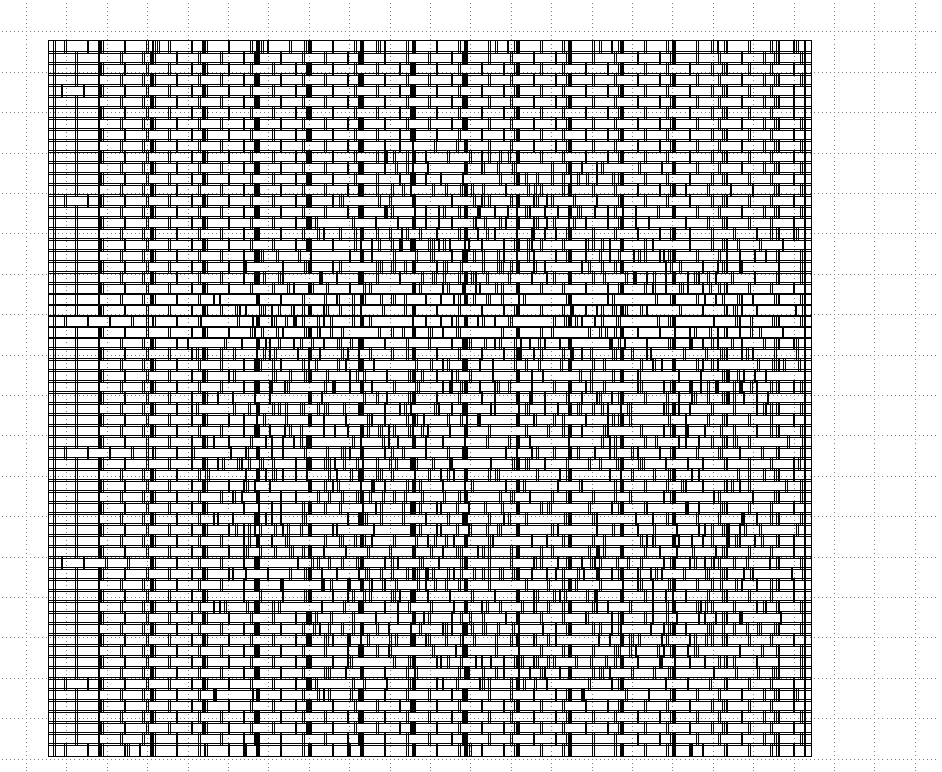
\includegraphics[width=0.72\textwidth]{figures/gds_rows.png}}

Hình~\ref{fig:gdsmet} là cùng đế với hai lớp kim loại đang bật. Dây xanh đi ngang. Dây tím đi dọc. Hình~\ref{fig:gdspanel} là cửa sổ KLayout của chính file đó: lớp đang chọn cho thấy \texttt{met1.drawing} (68/20) là xanh và \texttt{met2.drawing} (69/20) là tím. Vậy trên đế này \texttt{met1} đi ngang và \texttt{met2} đi dọc. Via là ô nhỏ nơi một dây đổi giữa hai lớp. Số 5571 là số via của cả đế trong báo cáo lần chạy, không phải số đếm bằng mắt trên ảnh.

\figframe{Hai lớp kim loại trên \texttt{cordic.gds}. Xanh là \texttt{met1}, đi ngang. Tím là \texttt{met2}, đi dọc.\label{fig:gdsmet}}{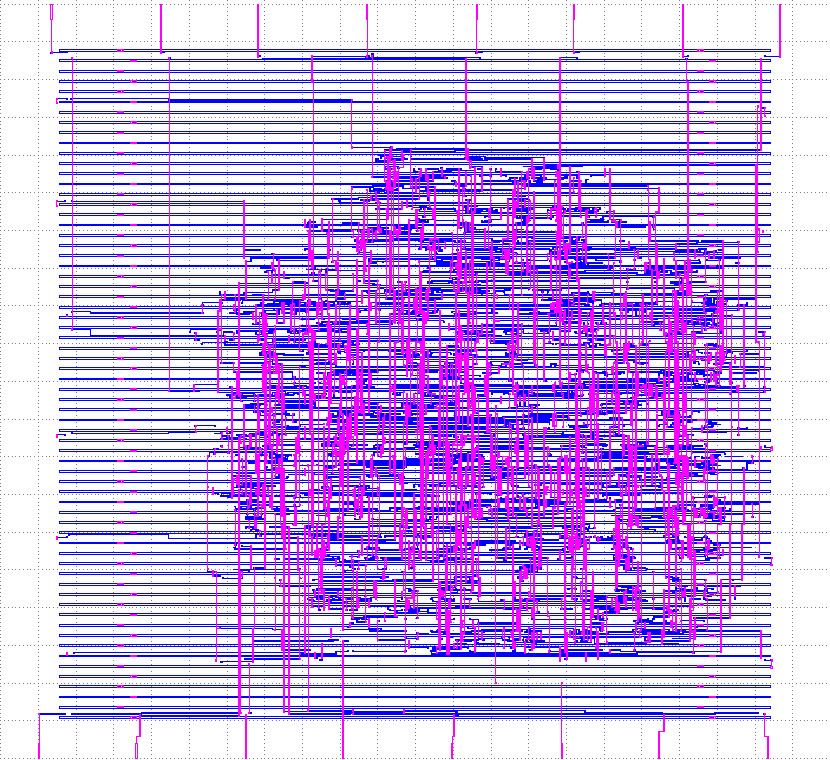
\includegraphics[width=0.78\textwidth]{figures/gds_metals.png}}

\figframe{Cửa sổ KLayout của \texttt{cordic.gds}, đỉnh \texttt{cordic}. Bảng lớp ghi \texttt{met1.drawing} màu xanh và \texttt{met2.drawing} màu tím.\label{fig:gdspanel}}{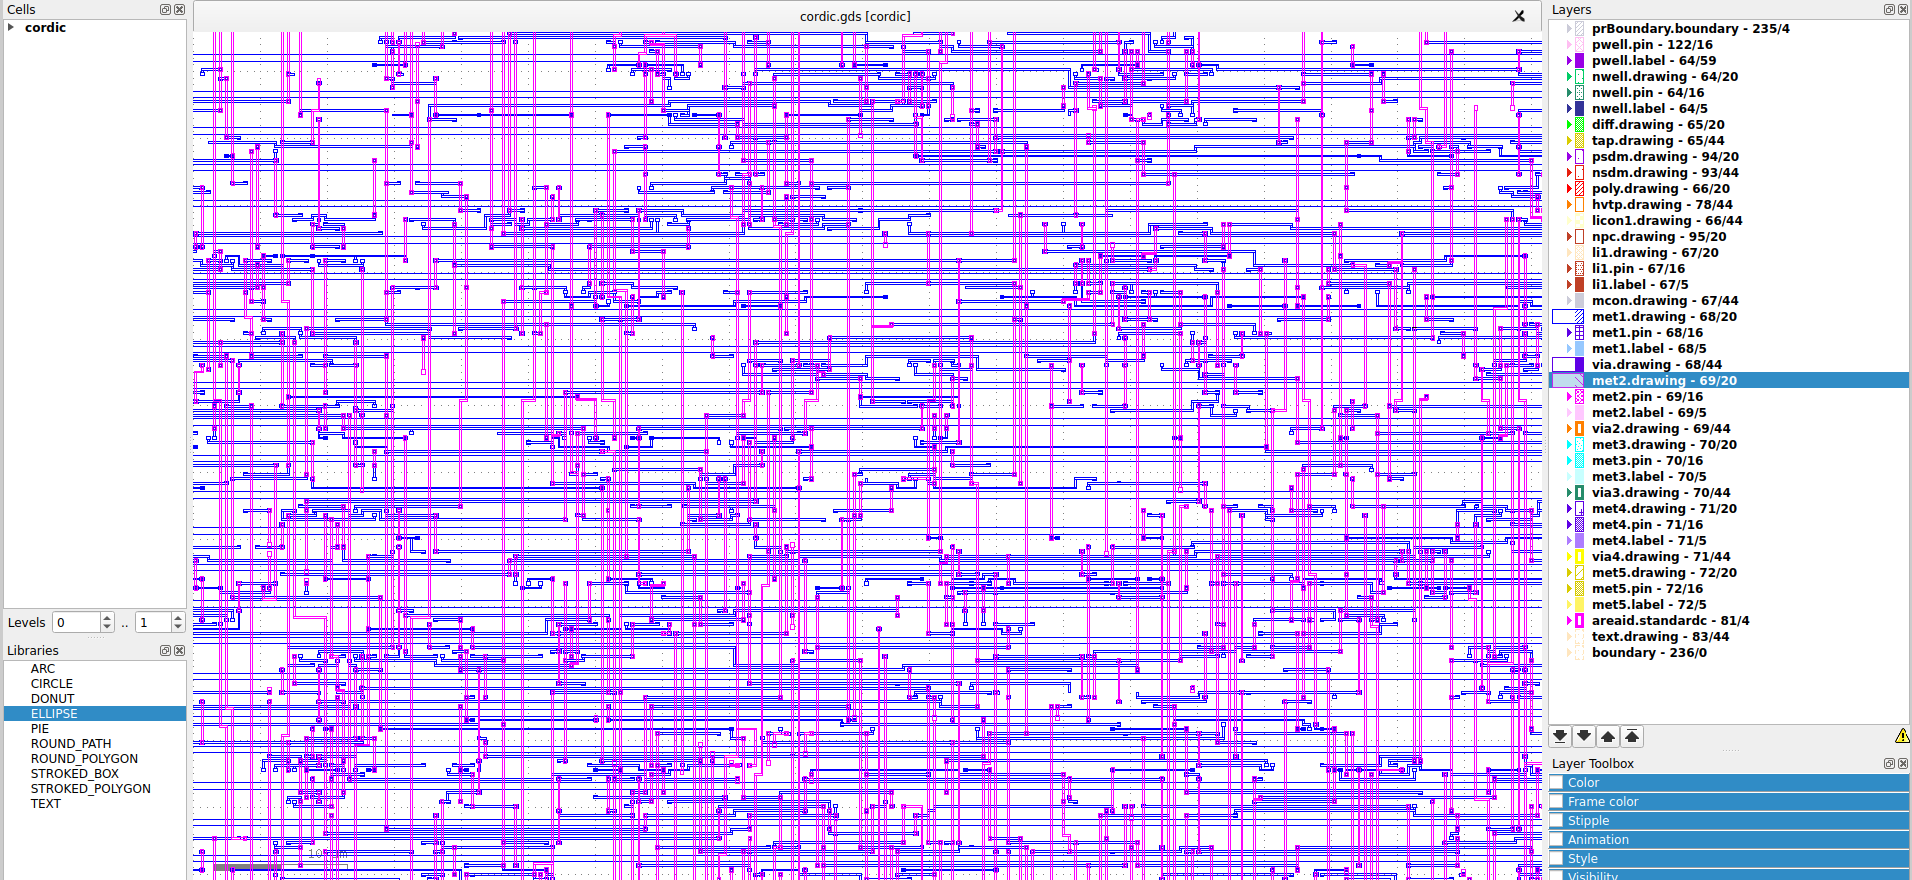
\includegraphics[width=0.92\textwidth]{figures/gds_panel.png}}

\subsection{Những gì nhìn thấy}

Đế là hình vuông cạnh \(200\,\mu\mathrm{m}\). Vùng giữa ảnh là các hàng cell, như Hình~\ref{fig:gdsrows}. Dây đã đi dài 23073 đơn vị của công cụ, với 5571 via. Hướng của hai lớp dưới đọc từ Hình~\ref{fig:gdsmet} và bảng lớp ở Hình~\ref{fig:gdspanel}: \texttt{met1} ngang, \texttt{met2} dọc. Chân trên đế là chân của lõi.

Phần lớn diện tích hàng không phải cổng của CORDIC. 755 cell logic nằm xen với 3146 filler, tap và decap. Nhìn trên ảnh, những mảnh đều trong hàng là các cell lấp chỗ. Cổng tính \texttt{sin} và \texttt{cos} là phần còn lại của cùng những hàng đó. Via là chỗ một dây đổi lớp kim loại. 5571 via là số lỗ như vậy trên cả đế, không phải số cổng.

\subsection{Liên hệ quy trình}

Hàng cell trên ảnh là chỗ công cụ đặt transistor và lỗ tiếp xúc, nhìn ở mức ảnh layout. Dây và via là các lớp kim loại xếp lên nhau. Nhận xét này đọc từ file GDSII. Nó không phải số đo của một mẻ chế tạo.

\subsection{Phương pháp của lần chạy}

Đi dây có hai cách thông dụng. Một cách là đi chi tiết ngay trên toàn đế. Cách kia là đi dây toàn cục trước, để chừa đường, rồi đi dây chi tiết. Lần chạy này dùng cách thứ hai của OpenLane. Kết quả của cách đó trên đế này là chiều dài dây 23073 đơn vị và 5571 via.

Nhịp cũng có hai cách. Sao là một đệm nối thẳng tới mọi flip-flop. Cây là đệm gốc rồi đệm lá. Lần chạy này dùng cây. Trên đường setup, \texttt{clk} vào \texttt{clkbuf\_0\_clk}, đệm gốc loại \texttt{clkbuf\_16}, fanout 8 trên \texttt{clknet\_0\_clk}. Đệm lá \texttt{clkbuf\_3\_6\_\_f\_clk} kéo 7 flip-flop. Một đệm lá khác, \texttt{clkbuf\_3\_2\_\_f\_clk}, kéo 11 tải trong khi giới hạn là 10.

Hàng cell có thể chèn tap, decap và filler bằng tay, hoặc để flow chèn sau khi đặt cell logic. Lần chạy này để flow chèn, vì \texttt{config.tcl} của thiết kế không ghi lưới tap. Mặc định sky130 được chép vào lần chạy: tap cách khoảng \(13\,\mu\mathrm{m}\), decap lấy bản rộng nhất còn vừa, filler bịt ô 1 và ô 2. Netlist cuối có 469 tap, 2103 decap và 574 filler.

Thời gian có thể ước lượng trước khi có dây, hoặc rút điện trở và tụ của dây đã đi rồi mới phân tích. Lần chạy này dùng cách sau. File \texttt{31-rcx\_sta} là phân tích đó: slack setup \(4{,}73\,\mathrm{ns}\), slack hold \(0{,}29\,\mathrm{ns}\).

Bảng 7.1 gắn những gì nhìn thấy trên các ảnh với bước đặt cell và bước đi dây. Đệm nhịp không được khoanh trên các ảnh này. Tên của nó nằm trong netlist.

\noindent\textbf{Bảng 7.1 — Quan sát layout}

\begin{tabularx}{\textwidth}{|Y|Y|Y|}
\hline
Nhìn thấy gì & Ở đâu trên hình & Liên hệ với bước quy trình nào \\ \hline
hàng standard cell & vệt ngang giữa Hình~\ref{fig:gdsrows} & đặt cell lên đế \\ \hline
\texttt{met1} đi ngang, \texttt{met2} đi dọc & Hình~\ref{fig:gdsmet}, tên lớp ở Hình~\ref{fig:gdspanel} & các lớp kim loại xếp chồng \\ \hline
5571 via & số của cả đế, không đếm trên ảnh & lỗ đổi lớp kim loại \\ \hline
đệm nhịp 11 tải & netlist, không khoanh trên ảnh & phân phối xung, chỉ có ở mạch tuần tự \\ \hline
\end{tabularx}

\section{Phần đóng góp của AI}

AI được dùng như một trợ lý khi viết báo cáo. AI không chạy lại flow và không tạo số liệu mới.

AI hỗ trợ trong việc chạy command, comment cho hình và kết quả chạy ra. AI gợi giải thích các bước chạy và gợi ý các tài nguyên để tìm hiểu sâu hơn về các lần chạy và kết quả.

\section{Kết luận, giới hạn và tự đánh giá}

\subsection{Điều kiện của kết luận}

Mọi số layout ở trên đến từ một lần chạy. Ảnh OpenLane là \texttt{ff5509f65b17} và process design kit (PDK) là \texttt{sky130A}. Chu kỳ ràng buộc là 10 ns và mật độ đặt mục tiêu là 0{,}45. \texttt{metrics.csv} ghi \texttt{OpenDP\_Util} bằng 23{,}41, tức mật độ lúc đặt cell, và ghi \texttt{Final\_Util} bằng \(-1\). Giá trị \(-1\) nghĩa là flow không lưu hệ số sử dụng sau khi đi dây. Diện tích lõi là \(33344{,}48\,\mu\mathrm{m}^{2}\) trên đế \(200\,\mu\mathrm{m}\times 200\,\mu\mathrm{m}\).

\subsection{Việc chưa có số}

Diện tích tách theo từng loại cell không có: file thống kê chỉ cho tổng diện tích lõi lúc tổng hợp, \(7553{,}49\,\mu\mathrm{m}^{2}\), với 672 cell, trong đó \texttt{dfrtp} xuất hiện 66 lần. Kho không có Actions. Log phép phá mạch nằm ở Bảng 3.2, ngày 26/10/2026. Bảng 9.1 chỉ kết luận từ số đã có.

\subsection{Điều không được kết luận}

Bảng 9.1 ghi mỗi kết luận cạnh điều kết luận đó không chứng minh. DRC bằng 0 không chứng minh chức năng. \(100\,\mathrm{MHz}\) không phải tần số đo trên chip. Mỗi hàng của bảng nhắc điều kiện đã tạo ra số đó.

\subsection{Chip không được chế tạo}

Lần chạy là layout cục bộ của lõi \texttt{cordic}. Chip không được chế tạo. Không có số nào trong báo cáo này là số đo trên silicon. Các kết luận ở Bảng 9.1 dừng ở mô phỏng và ở file layout.

\noindent\textbf{Bảng 9.1 — Kết luận có điều kiện}

\begin{tabularx}{\textwidth}{|Y|Y|Y|}
\hline
Kết luận & Điều kiện đã tạo ra nó & Điều này không chứng minh \\ \hline
tám bước, sai số sine tối đa 2, cosine tối đa 4 & mười mã, công thức \(128\sin\theta\), ngày 2026-10-04 & không phải mọi mã 0--255 \\ \hline
734 cell, 66 flip-flop, 0 nhân & map sky130, PDK \texttt{sky130A} & không phải diện tích đã tiết kiệm so với bộ nhân \\ \hline
\texttt{wns} = 0 ở 10 ns & dây đã đi, trễ chân 2 ns & không phải tần số đo trên chip \\ \hline
DRC 0, LVS sạch & Magic, cùng lần chạy & không phải chức năng đúng \\ \hline
\end{tabularx}

Bảng 9.2 ghi mức Khá cho đặc tả, tổng hợp và thời gian.

\noindent\begin{minipage}{\textwidth}
\noindent\textbf{Bảng 9.2 — Tự đánh giá}

\begin{tabularx}{\textwidth}{|Y|Y|Y|}
\hline
Tiêu chí & Mức & Lý do \\ \hline
1. Đặc tả và sơ đồ khối & Khá & bốn trạng thái, tám giả định, ba slide \texttt{top}, \texttt{pu}, \texttt{cu} \\ \hline
3. Đọc báo cáo tổng hợp & Khá & 66 khớp 66, có tổng diện tích \(7553{,}49\,\mu\mathrm{m}^{2}\), chưa tách theo loại cell \\ \hline
4. Đọc báo cáo thời gian & Khá & slack setup \(4{,}73\,\mathrm{ns}\), hold \(0{,}29\,\mathrm{ns}\), có tên hai đầu đường \\ \hline
\end{tabularx}
\end{minipage}

\appendix
\section{Mã nguồn RTL đầy đủ}

\noindent\texttt{cordic.v} — lõi \texttt{cordic}: \texttt{u\_proc} cạnh \texttt{u\_ctrl}

\begin{verbatim}
`default_nettype none
`timescale 1ns/1ps

// Top: control unit beside the processing unit.
// The processing unit contains Block B (z, sigma) and Block A (x, y).
module cordic (
    input  wire              clk,
    input  wire              rst_n,
    input  wire              start,
    input  wire       [7:0]  angle,
    output wire              done,
    output wire signed [7:0] sin,
    output wire signed [7:0] cos
);

    wire               load;
    wire               run;
    wire        [2:0]  i;
    wire signed [15:0] x, y;
    wire               sign_sin, sign_cos;

    cordic_control u_ctrl (
        .clk   (clk),
        .rst_n (rst_n),
        .start (start),
        .x        (x),
        .y        (y),
        .sign_sin (sign_sin),
        .sign_cos (sign_cos),
        .load     (load),
        .run   (run),
        .i     (i),
        .done  (done),
        .sin   (sin),
        .cos   (cos)
    );

    cordic_processing u_proc (
        .clk   (clk),
        .rst_n (rst_n),
        .load  (load),
        .run   (run),
        .i     (i),
        .angle (angle),
        .x        (x),
        .y        (y),
        .sign_sin (sign_sin),
        .sign_cos (sign_cos)
    );

endmodule
\end{verbatim}

\noindent\texttt{tt\_um\_cordic.v} — vỏ chân Tiny Tapeout, nối \texttt{ui\_in} và \texttt{uio\_in[0]} vào lõi

\begin{verbatim}
`default_nettype none
`timescale 1ns/1ps

// Tiny Tapeout shell. Charter pins, which his package named and did not draw.
//   ui_in[7:0]  angle
//   uio_in[0]   start
//   uo_out[7:0] sin
//   uio_out[7:0] cos
// clk and rst_n are the chip pins beside those 24.
// uio_in and uio_out are the same eight wires. They are inputs while the
// core is waiting, and they drive cos on the one cycle done is high.
// start is ignored on that cycle so cos[0] cannot look like a new start.
module tt_um_cordic (
    input  wire [7:0] ui_in,
    output wire [7:0] uo_out,
    input  wire [7:0] uio_in,
    output wire [7:0] uio_out,
    output wire [7:0] uio_oe,
    input  wire       ena,
    input  wire       clk,
    input  wire       rst_n
);

    wire              done;
    wire signed [7:0] sin;
    wire signed [7:0] cos;

    cordic u_core (
        .clk   (clk),
        .rst_n (rst_n),
        .start (uio_in[0] & ~done),
        .angle (ui_in),
        .done  (done),
        .sin   (sin),
        .cos   (cos)
    );

    assign uo_out  = sin;
    assign uio_out = cos;
    assign uio_oe  = done ? 8'hff : 8'h00;

    wire _unused = &{ena, uio_in[7:1], 1'b0};

endmodule
\end{verbatim}

\noindent\texttt{cordic\_control.v} — khối điều khiển trên slide \texttt{cu}

\begin{verbatim}
`default_nettype none
`timescale 1ns/1ps

// Control unit. State register, iteration register, and the output sample.
module cordic_control (
    input  wire               clk,
    input  wire               rst_n,
    input  wire               start,
    input  wire signed [15:0] x,
    input  wire signed [15:0] y,
    input  wire               sign_sin,
    input  wire               sign_cos,
    output wire               load,
    output wire               run,
    output wire        [2:0]  i,
    output wire               done,
    output wire signed [7:0]  sin,
    output wire signed [7:0]  cos
);
    localparam LOAD = 2'd1;
    localparam RUN  = 2'd2;

    wire [1:0] state;
    wire [1:0] state_next;
    wire [2:0] i_next;
    wire       sample;
    wire signed [7:0] x8, y8;
    wire signed [7:0] sin_cap, cos_cap;
    wire [7:0] sin_d, cos_d;
    wire       done_next;

    ctrl_next u_next (
        .state      (state),
        .i          (i),
        .start      (start),
        .state_next (state_next),
        .i_next     (i_next),
        .sample     (sample)
    );

    dreg #(.WIDTH(2)) u_state (
        .clk   (clk),
        .rst_n (rst_n),
        .d     (state_next),
        .q     (state)
    );

    dreg #(.WIDTH(3)) u_i (
        .clk   (clk),
        .rst_n (rst_n),
        .d     (i_next),
        .q     (i)
    );

    assign load = (state == LOAD);
    assign run  = (state == RUN);

    narrow_i8 u_cos (
        .v  (x),
        .y8 (x8)
    );

    narrow_i8 u_sin (
        .v  (y),
        .y8 (y8)
    );

    assign cos_cap = sign_cos ? -x8 : x8;
    assign sin_cap = sign_sin ? -y8 : y8;

    sample_mux u_cos_mux (
        .sample   (sample),
        .hold     (cos),
        .captured (cos_cap),
        .d        (cos_d)
    );

    sample_mux u_sin_mux (
        .sample   (sample),
        .hold     (sin),
        .captured (sin_cap),
        .d        (sin_d)
    );

    dreg #(.WIDTH(8)) u_cos_reg (
        .clk   (clk),
        .rst_n (rst_n),
        .d     (cos_d),
        .q     (cos)
    );

    dreg #(.WIDTH(8)) u_sin_reg (
        .clk   (clk),
        .rst_n (rst_n),
        .d     (sin_d),
        .q     (sin)
    );

    assign done_next = sample;
    dreg #(.WIDTH(1)) u_done (
        .clk   (clk),
        .rst_n (rst_n),
        .d     (done_next),
        .q     (done)
    );
endmodule
\end{verbatim}

\noindent\texttt{cordic\_processing.v} — khối xử lý trên slide \texttt{pu}

\begin{verbatim}
`default_nettype none
`timescale 1ns/1ps

// Processing unit. Block B produces sigma. Block A rotates x and y.
// load writes the starting values. run updates one iteration.
module cordic_processing (
    input  wire               clk,
    input  wire               rst_n,
    input  wire               load,
    input  wire               run,
    input  wire        [2:0]  i,
    input  wire        [7:0]  angle,
    output wire signed [15:0] x,
    output wire signed [15:0] y,
    output wire               sign_sin,
    output wire               sign_cos
);

    localparam signed [15:0] K_XY = 16'sd9949;  // 0.607253 * 16384

    wire              sigma;
    wire signed [9:0] z;
    wire signed [9:0] z_load;
    wire              sign_sin_now, sign_cos_now;
    wire              sign_sin_d, sign_cos_d;

    angle_fold u_angle (
        .angle    (angle),
        .z_load   (z_load),
        .sign_sin (sign_sin_now),
        .sign_cos (sign_cos_now)
    );

    // Captured with z, so a later change of angle does not flip the quadrant.
    assign sign_sin_d = load ? sign_sin_now : sign_sin;
    assign sign_cos_d = load ? sign_cos_now : sign_cos;
    dreg #(.WIDTH(1)) u_sign_sin (
        .clk   (clk),
        .rst_n (rst_n),
        .d     (sign_sin_d),
        .q     (sign_sin)
    );
    dreg #(.WIDTH(1)) u_sign_cos (
        .clk   (clk),
        .rst_n (rst_n),
        .d     (sign_cos_d),
        .q     (sign_cos)
    );

    cordic_block_b u_b (
        .clk    (clk),
        .rst_n  (rst_n),
        .load   (load),
        .run    (run),
        .i      (i),
        .z_load (z_load),
        .z      (z),
        .sigma  (sigma)
    );

    cordic_block_a u_a (
        .clk    (clk),
        .rst_n  (rst_n),
        .load   (load),
        .run    (run),
        .i      (i),
        .sigma  (sigma),
        .x_load (K_XY),
        .y_load (16'sd0),
        .x      (x),
        .y      (y)
    );

endmodule
\end{verbatim}

\noindent\texttt{cordic\_block\_a.v} — \texttt{u\_a}, cập nhật \texttt{x} và \texttt{y}

\begin{verbatim}
`default_nettype none
`timescale 1ns/1ps

// Block A: two shift blocks, two {load, run} muxes, two D registers.
module cordic_block_a (
    input  wire               clk,
    input  wire               rst_n,
    input  wire               load,
    input  wire               run,
    input  wire        [2:0]  i,
    input  wire               sigma,
    input  wire signed [15:0] x_load,
    input  wire signed [15:0] y_load,
    output wire signed [15:0] x,
    output wire signed [15:0] y
);
    wire        [1:0]  sel = {load, run};
    wire signed [15:0] x_rot, y_rot;
    wire signed [15:0] x_d, y_d;

    shift_block u_x_rot (
        .main_axis    (x),
        .sub_axis     (y),
        .i            (i),
        .sigma        (sigma),
        .add_on_sigma (1'b0),
        .result       (x_rot)
    );

    shift_block u_y_rot (
        .main_axis    (y),
        .sub_axis     (x),
        .i            (i),
        .sigma        (sigma),
        .add_on_sigma (1'b1),
        .result       (y_rot)
    );

    axis_mux u_x_mux (
        .sel     (sel),
        .hold    (x),
        .on_load (x_load),
        .on_run  (x_rot),
        .d       (x_d)
    );

    axis_mux u_y_mux (
        .sel     (sel),
        .hold    (y),
        .on_load (y_load),
        .on_run  (y_rot),
        .d       (y_d)
    );

    axis_reg u_x (
        .clk   (clk),
        .rst_n (rst_n),
        .d     (x_d),
        .q     (x)
    );

    axis_reg u_y (
        .clk   (clk),
        .rst_n (rst_n),
        .d     (y_d),
        .q     (y)
    );
endmodule
\end{verbatim}

\noindent\texttt{cordic\_block\_b.v} — \texttt{u\_b}, cập nhật \texttt{z}

\begin{verbatim}
`default_nettype none
`timescale 1ns/1ps

// Block B: angle table, add/sub, {load, run} mux, z register, sigma.
module cordic_block_b (
    input  wire               clk,
    input  wire               rst_n,
    input  wire               load,
    input  wire               run,
    input  wire        [2:0]  i,
    input  wire signed [9:0] z_load,
    output wire signed [9:0] z,
    output wire              sigma
);
    wire       [1:0] sel = {load, run};
    wire       [9:0] alpha_u;
    wire signed [9:0] alpha;
    wire signed [9:0] z_rot;
    wire signed [9:0] z_d;

    atan_lut u_lut (
        .i     (i),
        .alpha (alpha_u)
    );
    assign alpha = $signed(alpha_u);

    addsub_block #(.WIDTH(10)) u_z_rot (
        .main_axis    (z),
        .sub_axis     (alpha),
        .sigma        (sigma),
        .add_on_sigma (1'b0),
        .result       (z_rot)
    );

    axis_mux #(.WIDTH(10)) u_z_mux (
        .sel     (sel),
        .hold    (z),
        .on_load (z_load),
        .on_run  (z_rot),
        .d       (z_d)
    );

    axis_reg #(.WIDTH(10)) u_z (
        .clk   (clk),
        .rst_n (rst_n),
        .d     (z_d),
        .q     (z)
    );

    sigma_block u_sigma (
        .z     (z),
        .sigma (sigma)
    );
endmodule
\end{verbatim}

\noindent\texttt{cordic\_cells.v} — \texttt{ctrl\_next}, \texttt{axis\_mux}, \texttt{addsub\_block}, \texttt{atan\_lut}, \texttt{axis\_reg}

\begin{verbatim}
`default_nettype none
`timescale 1ns/1ps

// D flip-flop. The one leaf that stores a value.
module dreg #(
    parameter integer WIDTH = 1
) (
    input  wire                  clk,
    input  wire                  rst_n,
    input  wire [WIDTH-1:0]      d,
    output reg  [WIDTH-1:0]      q
);
    always @(posedge clk or negedge rst_n) begin
        if (!rst_n)
            q <= {WIDTH{1'b0}};
        else
            q <= d;
    end
endmodule

// Datapath register. Same cell as dreg, signed ports. x and y use 16. z uses 10.
module axis_reg #(
    parameter integer WIDTH = 16
) (
    input  wire                    clk,
    input  wire                    rst_n,
    input  wire signed [WIDTH-1:0] d,
    output wire signed [WIDTH-1:0] q
);
    dreg #(.WIDTH(WIDTH)) u_ff (
        .clk   (clk),
        .rst_n (rst_n),
        .d     (d),
        .q     (q)
    );
endmodule

// sel is {load, run}. load wins when both are 1.
module axis_mux #(
    parameter integer WIDTH = 16
) (
    input  wire        [1:0]       sel,
    input  wire signed [WIDTH-1:0] hold,
    input  wire signed [WIDTH-1:0] on_load,
    input  wire signed [WIDTH-1:0] on_run,
    output wire signed [WIDTH-1:0] d
);
    assign d = sel[1] ? on_load :
               sel[0] ? on_run  :
                        hold;
endmodule

// main +/- sub. add_on_sigma 1 adds when sigma is 1.
module addsub_block #(
    parameter integer WIDTH = 16
) (
    input  wire signed [WIDTH-1:0] main_axis,
    input  wire signed [WIDTH-1:0] sub_axis,
    input  wire                    sigma,
    input  wire                    add_on_sigma,
    output wire signed [WIDTH-1:0] result
);
    wire do_add = sigma ~^ add_on_sigma;
    assign result = do_add ? (main_axis + sub_axis) : (main_axis - sub_axis);
endmodule

// main +/- (sub >>> i). The x path uses add_on_sigma 0, the y path uses 1.
module shift_block (
    input  wire signed [15:0] main_axis,
    input  wire signed [15:0] sub_axis,
    input  wire        [2:0]  i,
    input  wire               sigma,
    input  wire               add_on_sigma,
    output wire signed [15:0] result
);
    wire signed [15:0] sub_shr = sub_axis >>> i;
    addsub_block u_as (
        .main_axis    (main_axis),
        .sub_axis     (sub_shr),
        .sigma        (sigma),
        .add_on_sigma (add_on_sigma),
        .result       (result)
    );
endmodule

// arctan(2^-i) in brads. 256 counts = 360 degrees. The last entry underflows to 0.
module atan_lut (
    input  wire       [2:0] i,
    output reg        [9:0] alpha
);
    always @* begin
        case (i)
            3'd0: alpha = 10'd32;
            3'd1: alpha = 10'd19;
            3'd2: alpha = 10'd10;
            3'd3: alpha = 10'd5;
            3'd4: alpha = 10'd3;
            3'd5: alpha = 10'd1;
            3'd6: alpha = 10'd1;
            default: alpha = 10'd0;
        endcase
    end
endmodule

// sigma = 1 when z is positive or zero.
module sigma_block (
    input  wire signed [9:0] z,
    output wire              sigma
);
    assign sigma = (z >= 0);
endmodule

// Fold one brad byte into the first quadrant and remember which quadrant it came from.
// 0..63, 64..127, 128..191, 192..255. z_load stays in 0..64.
module angle_fold (
    input  wire        [7:0] angle,
    output reg  signed [9:0] z_load,
    output reg               sign_sin,
    output reg               sign_cos
);
    always @* begin
        z_load   = 10'sd0;
        sign_cos = 1'b0;
        sign_sin = 1'b0;
        if (angle < 8'd64) begin
            z_load   = $signed({2'b00, angle});
            sign_cos = 1'b0;
            sign_sin = 1'b0;
        end else if (angle < 8'd128) begin
            z_load   = $signed({2'b00, (8'd128 - angle)});
            sign_cos = 1'b1;
            sign_sin = 1'b0;
        end else if (angle < 8'd192) begin
            z_load   = $signed({2'b00, (angle - 8'd128)});
            sign_cos = 1'b1;
            sign_sin = 1'b1;
        end else begin
            z_load   = $signed(10'd256 - {2'b00, angle});
            sign_cos = 1'b0;
            sign_sin = 1'b1;
        end
    end
endmodule

// 16-bit x,y with 1.0 at bit 14 -> 8-bit pin with 1.0 at bit 7.
module narrow_i8 (
    input  wire signed [15:0] v,
    output reg  signed [7:0]  y8
);
    reg signed [15:0] t;
    always @* begin
        t = v >>> 7;
        if (t > 16'sd127)
            y8 = 8'sd127;
        else if (t < -16'sd128)
            y8 = -8'sd128;
        else
            y8 = t[7:0];
    end
endmodule

// Pick the new 8-bit pin on the sample cycle, otherwise hold.
module sample_mux (
    input  wire       sample,
    input  wire [7:0] hold,
    input  wire [7:0] captured,
    output wire [7:0] d
);
    assign d = sample ? captured : hold;
endmodule

// Next state and next iteration. Combinational only.
module ctrl_next (
    input  wire [1:0] state,
    input  wire [2:0] i,
    input  wire       start,
    output reg  [1:0] state_next,
    output reg  [2:0] i_next,
    output wire       sample
);
    localparam IDLE   = 2'd0;
    localparam LOAD   = 2'd1;
    localparam RUN    = 2'd2;
    localparam SAMPLE = 2'd3;

    assign sample = (state == SAMPLE);

    always @* begin
        state_next = state;
        i_next     = i;
        case (state)
            IDLE: begin
                if (start) begin
                    state_next = LOAD;
                    i_next     = 3'd0;
                end
            end
            LOAD: state_next = RUN;
            RUN: begin
                if (i == 3'd7)
                    state_next = SAMPLE;
                else
                    i_next = i + 3'd1;
            end
            SAMPLE: state_next = IDLE;
            default: state_next = IDLE;
        endcase
    end
endmodule
\end{verbatim}

\section{Testbench đầy đủ}

\noindent\texttt{tb\_cordic.v} — testbench của lõi, in \texttt{I05 RTL TB PASS}

\begin{verbatim}
`timescale 1ns/1ps
// Same check as i05_cordic_core_tb.sv. Stored integers, pass band +/- 4.
// Port names follow this design: sin, cos, done. There is no busy pin.
module tb_cordic;
    reg clk = 0, rst_n = 0, start = 0;
    reg [7:0] angle;
    wire signed [7:0] sin, cos;
    wire done;

    cordic dut (
        .clk   (clk),
        .rst_n (rst_n),
        .start (start),
        .angle (angle),
        .sin   (sin),
        .cos   (cos),
        .done  (done)
    );

    always #5 clk = ~clk;

    task run_case;
        input [7:0] p;
        input integer sin_expected;
        input integer cos_expected;
        integer ds, dc;
        begin
            @(negedge clk);
            angle = p;
            start = 1'b1;

            @(negedge clk);
            start = 1'b0;

            wait (done);

            ds = sin - sin_expected;
            dc = cos - cos_expected;

            if ((ds > 4) || (ds < -4))
                $fatal(1, "sin mismatch p=%0d got=%0d exp=%0d", p, sin, sin_expected);
            if ((dc > 4) || (dc < -4))
                $fatal(1, "cos mismatch p=%0d got=%0d exp=%0d", p, cos, cos_expected);
        end
    endtask

    initial begin
        angle = 0;

        repeat (2) @(posedge clk);
        rst_n = 1;

        run_case(8'd0,    0,   127);
        run_case(8'd64,   127,   0);
        run_case(8'd128,  0,  -128);
        run_case(8'd192, -128,   0);
        run_case(8'd32,   91,   91);
        run_case(8'd224, -91,   91);

        $display("I05 RTL TB PASS");
        $finish;
    end
endmodule
\end{verbatim}

\noindent\texttt{tb\_tt\_um\_cordic.v} — testbench của vỏ chân, in \texttt{I05 PIN SHELL PASS}

\begin{verbatim}
`timescale 1ns/1ps
// Same six cases and the same +/- 4 band as i05_cordic_core_tb.sv,
// read back through the charter pins.
module tb_tt_um_cordic;
    reg clk = 0, rst_n = 0, ena = 1;
    reg [7:0] ui_in;
    reg [7:0] uio_in;
    wire [7:0] uo_out, uio_out, uio_oe;

    tt_um_cordic dut (
        .ui_in   (ui_in),
        .uo_out  (uo_out),
        .uio_in  (uio_in),
        .uio_out (uio_out),
        .uio_oe  (uio_oe),
        .ena     (ena),
        .clk     (clk),
        .rst_n   (rst_n)
    );

    always #5 clk = ~clk;

    task run_case;
        input [7:0] p;
        input integer sin_expected;
        input integer cos_expected;
        integer ds, dc;
        begin
            @(negedge clk);
            ui_in  = p;
            uio_in = 8'b0000_0001;

            @(negedge clk);
            uio_in = 8'b0;

            wait (uio_oe == 8'hff);

            ds = $signed(uo_out) - sin_expected;
            dc = $signed(uio_out) - cos_expected;

            if ((ds > 4) || (ds < -4))
                $fatal(1, "sin mismatch p=%0d got=%0d exp=%0d", p, $signed(uo_out), sin_expected);
            if ((dc > 4) || (dc < -4))
                $fatal(1, "cos mismatch p=%0d got=%0d exp=%0d", p, $signed(uio_out), cos_expected);

            @(posedge clk);
            @(negedge clk);
            if (uio_oe != 8'h00)
                $fatal(1, "uio stayed an output after done, p=%0d oe=%b", p, uio_oe);
        end
    endtask

    initial begin
        ui_in = 0;
        uio_in = 0;

        repeat (2) @(posedge clk);
        rst_n = 1;

        run_case(8'd0,    0,   127);
        run_case(8'd64,   127,   0);
        run_case(8'd128,  0,  -128);
        run_case(8'd192, -128,   0);
        run_case(8'd32,   91,   91);
        run_case(8'd224, -91,   91);

        $display("I05 PIN SHELL PASS");
        $finish;
    end
endmodule
\end{verbatim}

\noindent\texttt{tb\_error\_dump.v} — đổ sai số của mười mã

\begin{verbatim}
`timescale 1ns/1ps
// Print chip sin/cos for the error table. This file does not replace tb_cordic.v.
// The true sin/cos codes are computed in error_table.py. No pi in this bench.
module tb_error_dump;
    reg clk = 0, rst_n = 0, start = 0;
    reg [7:0] angle;
    wire signed [7:0] sin, cos;
    wire done;

    cordic dut (
        .clk   (clk),
        .rst_n (rst_n),
        .start (start),
        .angle (angle),
        .sin   (sin),
        .cos   (cos),
        .done  (done)
    );

    always #5 clk = ~clk;

    task dump_case;
        input [7:0] p;
        begin
            @(negedge clk);
            angle = p;
            start = 1'b1;
            @(negedge clk);
            start = 1'b0;
            wait (done);
            $display("CHIP %0d %0d %0d", p, sin, cos);
        end
    endtask

    initial begin
        angle = 0;
        repeat (2) @(posedge clk);
        rst_n = 1;

        dump_case(8'd0);
        dump_case(8'd21);
        dump_case(8'd32);
        dump_case(8'd43);
        dump_case(8'd64);
        dump_case(8'd96);
        dump_case(8'd128);
        dump_case(8'd192);
        dump_case(8'd224);
        dump_case(8'd255);

        $finish;
    end
endmodule
\end{verbatim}

\noindent\texttt{tb\_gtkwave.v} — một lần tính mã 32 cho dạng sóng

\begin{verbatim}
`timescale 1ns/1ps
// One sample for GTKWave. Angle code 32 is 45 degrees.
// States: 0 Cho, 1 Nap, 2 Quay, 3 Lay mau.
// Open gtkwave on gtkwave/fsm_45.vcd and show:
//   clk start rst_n state i x y z sigma sin cos done
module tb_gtkwave;
    reg clk = 0, rst_n = 0, start = 0;
    reg [7:0] angle;
    wire signed [7:0] sin, cos;
    wire done;

    cordic dut (
        .clk   (clk),
        .rst_n (rst_n),
        .start (start),
        .angle (angle),
        .sin   (sin),
        .cos   (cos),
        .done  (done)
    );

    wire [1:0] state = dut.u_ctrl.u_state.q;
    wire [2:0] i     = dut.u_ctrl.u_i.q;
    wire signed [15:0] x = dut.u_proc.u_a.x;
    wire signed [15:0] y = dut.u_proc.u_a.y;
    wire signed [9:0]  z = dut.u_proc.u_b.z;
    wire sigma = dut.u_proc.u_b.sigma;

    always #5 clk = ~clk;

    function [8*8-1:0] sname;
        input [1:0] s;
        begin
            case (s)
                2'd0: sname = "Cho";
                2'd1: sname = "Nap";
                2'd2: sname = "Quay";
                2'd3: sname = "Lay mau";
                default: sname = "?";
            endcase
        end
    endfunction

    initial begin
        $dumpfile("gtkwave/fsm_45.vcd");
        $dumpvars(0, tb_gtkwave);
        angle = 8'd32;
        repeat (2) @(posedge clk);
        rst_n = 1;
        @(negedge clk);
        start = 1'b1;
        @(negedge clk);
        start = 1'b0;
        wait (done);
        @(posedge clk);
        @(posedge clk);
        $finish;
    end

    always @(posedge clk) begin
        #1;
        $display("t=%0t state=%s i=%0d sigma=%0b x=%0d y=%0d z=%0d sin=%0d cos=%0d done=%0b start=%0b",
                 $time, sname(state), i, sigma, x, y, z, sin, cos, done, start);
    end
endmodule
\end{verbatim}

\section{Thông tin tái lập}
\begin{tabularx}{\textwidth}{|l|Y|}
\hline
Đường dẫn kho GitHub & \url{https://github.com/haiminhtruongisavailable/I05_Intro_to_chip_design_project} \\ \hline
Mã commit dùng cho báo cáo & \texttt{0520dd2} \\ \hline
Số hiệu / đường dẫn lần chạy CI & không có Actions trên kho này \\ \hline
Phiên bản LibreLane & OpenLane image \texttt{ff5509f65b17}, lệnh \texttt{./flow.tcl -design cordic} \\ \hline
Phiên bản PDK & \texttt{sky130A} \\ \hline
Ràng buộc chu kỳ xung nhịp & 10 ns, trễ chân 2 ns \\ \hline
Ngày chạy & 03/10/2026, bảng sai số 04/10/2026 \\ \hline
Công cụ trí tuệ nhân tạo (AI) đã dùng và dùng vào việc gì & mô hình ngôn ngữ viết câu từ nhật ký lệnh của mạch này. Số liệu lấy từ lần chạy đã ghi. \\ \hline
\end{tabularx}

\section*{Cam kết}
Tôi xin cam đoan báo cáo này do tôi tự thực hiện. Toàn bộ số liệu trong báo cáo lấy từ lần chạy trên kho GitHub cá nhân nêu ở trang bìa và có thể đối chiếu được. Tôi hiểu rằng học phần này không thực hiện chế tạo chip, và các kết quả trong báo cáo là kết quả chạy công cụ mô phỏng và tổng hợp, không phải kết quả đo trên silicon.

\begin{flushleft}
Ngày \ldots\ tháng \ldots\ năm 20\ldots\\[1.2em]
Người thực hiện\\[4em]
(Ký và ghi rõ họ tên)
\end{flushleft}

\end{document}
